\documentclass[a4paper, 10pt, twoside]{article}

\usepackage[top=1in, bottom=1in, left=1in, right=1in]{geometry}
\usepackage[utf8]{inputenc}
\usepackage[spanish, es-ucroman, es-noquoting]{babel}
\usepackage{setspace}
\usepackage{fancyhdr}
\usepackage{lastpage}
\usepackage{amsmath}
\usepackage{amsfonts}
\usepackage{amsthm}
\usepackage{verbatim}
\usepackage{graphicx}
\usepackage{float}
\usepackage[noend]{algpseudocode}
\usepackage{enumitem} % Provee macro \setlist
\usepackage{tabularx}
\usepackage{multirow}
\usepackage[toc, page]{appendix}


%%%%%%%%%% Configuración de Fancyhdr - Inicio %%%%%%%%%%
\pagestyle{fancy}
\thispagestyle{fancy}
\lhead{Trabajo Práctico 3 · Algoritmos y Estructuras de Datos III}
\rhead{Lovisolo · Petaccio · Rossi}
\renewcommand{\footrulewidth}{0.4pt}
\cfoot{\thepage /\pageref{LastPage}}

\fancypagestyle{caratula} {
   \fancyhf{}
   \cfoot{\thepage /\pageref{LastPage}}
   \renewcommand{\headrulewidth}{0pt}
   \renewcommand{\footrulewidth}{0pt}
}
%%%%%%%%%% Configuración de Fancyhdr - Fin %%%%%%%%%%


%%%%%%%%%% Configuración de Algorithmic - Inicio %%%%%%%%%%
% Entorno propio para customizar la presentación del pseudocódigo
\newenvironment{pseudo}[1][]{%
    \vspace{1em}%
    \begin{algorithmic}%
}
{%
    \end{algorithmic}%
    \vspace{1em}%
}


% switch
\algnewcommand\algorithmicswitch{\textbf{switch}}
\algnewcommand\algorithmiccase{\textbf{case}}
\algnewcommand\algorithmicassert{\texttt{assert}}
\algdef{SE}[SWITCH]{Switch}{EndSwitch}[1]{\algorithmicswitch\ #1\ \algorithmicdo}{\algorithmicend\ \algorithmicswitch}%
\algdef{SE}[CASE]{Case}{EndCase}[1]{\algorithmiccase\ #1}{\algorithmicend\ \algorithmiccase}%
\algtext*{EndSwitch}%
\algtext*{EndCase}%




% Valores de verdad
\newcommand{\True}{\textbf{true}}
\newcommand{\False}{\textbf{false}}

% Conectivos lógicos
\newcommand{\PAnd}{\textbf{and} }
\newcommand{\POr}{\textbf{or} }

% Conectivo 'in' para usar así: \ForAll{$foo$ \In $bar$}
\newcommand{\In}{\textbf{in} }

% Conectivo 'to' para usar así: \For{$i = 1$ \In $n$}
\newcommand{\To}{\textbf{to} }

% Control de flujo
\newcommand{\Break}{\State \textbf{break}}
\newcommand{\PReturn}{\State \textbf{return} }

% Complejidades
\newcommand{\Ode}[1]{\hfill $O(#1)$}
%%%%%%%%%% Configuración de Algorithmic - Fin %%%%%%%%%%


%%%%%%%%%% Miscelánea - Inicio %%%%%%%%%%
% Evita que el documento se estire verticalmente para ocupar el espacio vacío
% en cada página.
\raggedbottom

% Deshabilita sangría en la primer línea de un párrafo.
\setlength{\parindent}{0em}

% Separación entre párrafos.
\setlength{\parskip}{0.5em}

% Separación entre elementos de listas.
\setlist{itemsep=0.5em}

% Asigna la traducción de la palabra 'Appendices'.
\renewcommand{\appendixtocname}{Apéndices}
\renewcommand{\appendixpagename}{Apéndices}
%%%%%%%%%% Miscelánea - Fin %%%%%%%%%%


%%%%%%%%%% Gráficos - Inicio %%%%%%%%%%
% Macro para incluir tres gráficos (dentro de una figura) de manera que
% entren todos en una sola página.
\newcommand{\tresgraficos}[3]{
    \newcommand{\separacion}{-2.2em}
    \vspace{\separacion}
    \include{#1}
    \vspace{\separacion}
    \include{#2}
    \vspace{\separacion}
    \include{#3}
}

% Macro para incluir dos gráficos (dentro de una figura) de manera que
% entren todos en una sola página.
\newcommand{\dosgraficos}[2]{
    \newcommand{\separacion}{-2.2em}
    \vspace{\separacion}
    \include{#1}
    \vspace{\separacion}
    \include{#2}
}
%%%%%%%%%% Gráficos - Fin %%%%%%%%%%


\begin{document}


%%%%%%%%%%%%%%%%%%%%%%%%%%%%%%%%%%%%%%%%%%%%%%%%%%%%%%%%%%%%%%%%%%%%%%%%%%%%%%%
%% Carátula                                                                  %%
%%%%%%%%%%%%%%%%%%%%%%%%%%%%%%%%%%%%%%%%%%%%%%%%%%%%%%%%%%%%%%%%%%%%%%%%%%%%%%%


\thispagestyle{caratula}

\begin{center}


\includegraphics[height=2cm]{DC.png} 
\hfill

\includegraphics[height=2cm]{UBA.jpg} 

\vspace{2cm}

Departamento de Computación,\\
Facultad de Ciencias Exactas y Naturales,\\
Universidad de Buenos Aires

\vspace{4cm}

\begin{Huge}
Trabajo Práctico 3
\end{Huge}

\vspace{0.5cm}

\begin{Large}
Algoritmos y Estructuras de Datos III
\end{Large}

\vspace{1cm}

Segundo Cuatrimestre de 2013

\vspace{4cm}

\begin{tabular}{|c|c|c|}
\hline
Apellido y Nombre & LU & E-mail\\
\hline
Leandro Lovisolo      & 645/11 & leandro@leandro.me\\
Lautaro José Petaccio & 443/11 & lausuper@gmail.com\\
Lucas Rossi           & 705/11 & lucasrossi20@gmail.com\\
\hline
\end{tabular}

\end{center}

\newpage


%%%%%%%%%%%%%%%%%%%%%%%%%%%%%%%%%%%%%%%%%%%%%%%%%%%%%%%%%%%%%%%%%%%%%%%%%%%%%%%
%% Índice                                                                    %%
%%%%%%%%%%%%%%%%%%%%%%%%%%%%%%%%%%%%%%%%%%%%%%%%%%%%%%%%%%%%%%%%%%%%%%%%%%%%%%%


\tableofcontents

\newpage


%%%%%%%%%%%%%%%%%%%%%%%%%%%%%%%%%%%%%%%%%%%%%%%%%%%%%%%%%%%%%%%%%%%%%%%%%%%%%%%
%% Introducción                                                              %%
%%%%%%%%%%%%%%%%%%%%%%%%%%%%%%%%%%%%%%%%%%%%%%%%%%%%%%%%%%%%%%%%%%%%%%%%%%%%%%%


\section{Introducción}

En el presente trabajo estudiamos tres problemas algorítmicos, proponemos soluciones para los mismos respetando sus requerimientos de complejidad temporal y analizamos empíricamente los tiempos de ejecución de sus implementaciones en lenguaje C++.

La motivación de este trabajo es comparar las cotas temporales obtenidas del análisis teórico con las mediciones de tiempos de ejecución y extraer conclusiones de esta experimentación.

Sin más, presentamos los problemas estudiados a continuación.


%%%%%%%%%%%%%%%%%%%%%%%%%%%%%%%%%%%%%%%%%%%%%%%%%%%%%%%%%%%%%%%%%%%%%%%%%%%%%%%
%% Descipcion de situaciones reales                                          %%
%%%%%%%%%%%%%%%%%%%%%%%%%%%%%%%%%%%%%%%%%%%%%%%%%%%%%%%%%%%%%%%%%%%%%%%%%%%%%%%


\newpage

\section{Descripción de situaciones reales}
\begin{itemize}
\item Un área perteneciente a un bosque quiere abrirse a turistas. El bosque tiene una serie de senderos (aristas) que lo recorren y una serie de espacios libres (nodos). Los guardabosques quieren que la gente no se pierda nada de la naturaleza del bosque, quieren que los turistas puedan recorrer la mayor cantidad de caminos posibles. Como la gente es muy vaga, solo recorre los caminos que estén conectados a un claro donde haya un puesto para bebidas y descanso. Es necesario que los puestos estén todos comunicados para poder proveerse entre sí en caso de que a alguno le falte algo o necesite ayuda. 

Mediante el algoritmo de CFM podemos encontrar los espacios libres conectados entre sí para poner los paradores de manera que la gente pueda recorrer la mayor cantidad posible de caminos del bosque sin cansarse tanto.

\item Se tiene en una ciudad una serie de plantas potabilizadoras (nodos) y cañerías (aristas) por donde circula el agua sucia. Se quiere poder buscar un conjunto de plantas adyacentes, ya que estando adyacentes será posible tratar en común los desechos obtenidos para producir energía, que tenga una cantidad máxima de cañerías que se comuniquen con este conjunto para poder aprovechar la energía generada al máximo y potabilizar una gran cantidad de agua.

Utilizando el algoritmo de CFM es posible determinar que plantas seran las ideales para ubicar el generador de energía y poder potabilizar una gran parte del agua de la ciudad sin consumir energía de fuentes externas.
\end{itemize}


%%%%%%%%%%%%%%%%%%%%%%%%%%%%%%%%%%%%%%%%%%%%%%%%%%%%%%%%%%%%%%%%%%%%%%%%%%%%%%%
%% Familias de grafos utilizadas en este trabajo                             %%
%%%%%%%%%%%%%%%%%%%%%%%%%%%%%%%%%%%%%%%%%%%%%%%%%%%%%%%%%%%%%%%%%%%%%%%%%%%%%%%


\newpage
\section{Familias de grafos utilizadas en este trabajo}
\subsection{Kn U claw}
La familia consiste en un grafo Kn y un grafo claw o estrella formado por un nodo y m nodos adyacentes, 
unidos de forma disjunta, que es luego complementado.
\begin{figure}[H]
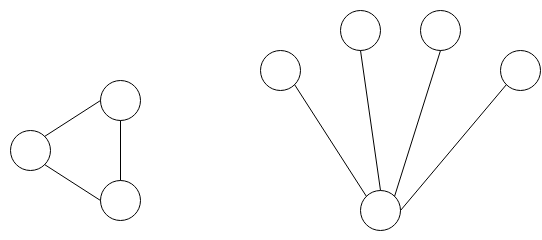
\includegraphics[width=80mm]{K3UC4.png}
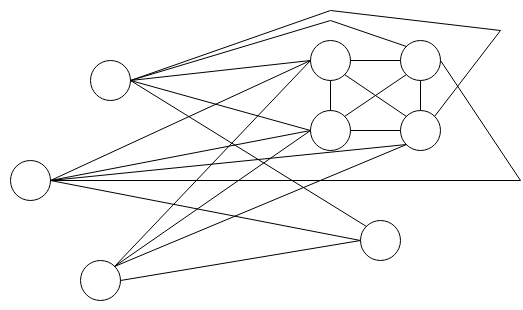
\includegraphics[width=80mm]{K3UC4Complemento.png}
\caption{La figura de la izquierda corresponde a K3 U claw 4, la figura derecha K3 U claw 4 complemento}
\label{overflow}
\end{figure}

\subsection{Grafo Completo K_n}
Un grafo completo es un grafo simple donde cada par de vértices está conectado por una arista.
Un grafo completo de n vértices tiene n(n-1)/2 aristas.
Es un grafo regular con todos sus vértices de grado n-1.

\begin{figure}[H]
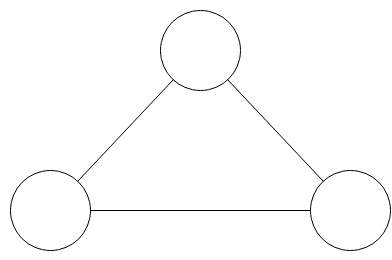
\includegraphics[width=80mm]{K3.png}
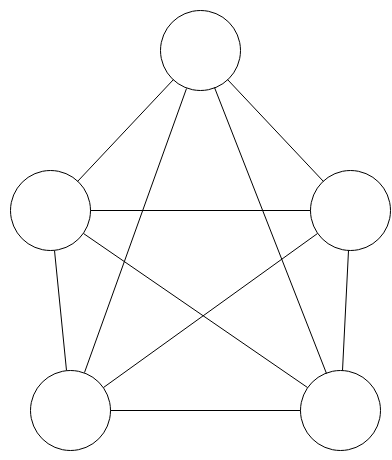
\includegraphics[width=80mm]{K5.png}
\caption{La figura de la izquierda corresponde a un grafo K_3 y la figura derecha a un grafo K_5}
\label{overflow}
\end{figure}

\subsection{Grafo Bipartito Completo K_n,_m}
Un grafo bipartito completo es aquel grafo bipartito en el que todos los vértices de la partición V_1 están conectados a todos los vértices de la partición V_2 y viceversa.

Donde un grafo bipartito es un grafo G=(V,E) cuyos vértices se pueden separar en dos conjuntos disjuntos V_1 y V_2, es decir, tal que se cumple:
V_1 $\cup$ V_2 = V
V_1 $\cap$ V_2 = $\emptyset$
de manera que las aristas sólo pueden conectar vértices de un conjunto con vértices del otro; es decir:
$\forall$ u_1,u_2 \in V_1, \forall v_1,v_2 \in V_2 no existe ninguna arista e=(u_1,u_2) ni e=(v_1,v_2).

\begin{figure}[H]
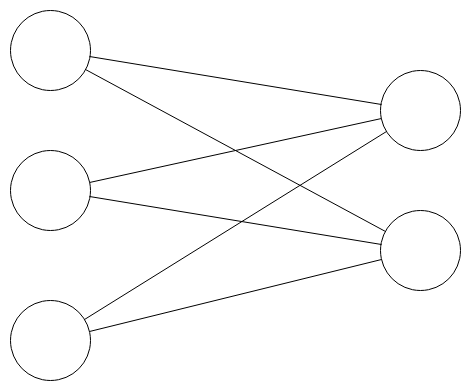
\includegraphics[width=80mm]{K3_2.png}
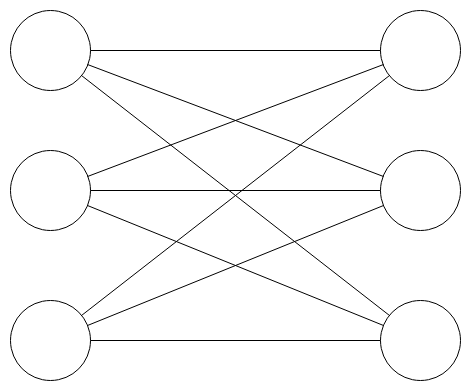
\includegraphics[width=80mm]{K3_3.png}
\caption{La figura de la izquierda corresponde a un grafo bipartito completo K_3_2 y la figura derecha a un grafo bipartito completo K_3_3}
\label{overflow}
\end{figure}


\subsection{Grafo Lattice L_m_n}
Un grafo Lattice es el producto cartesiano de dos grafos completos K_m y K_n.

\begin{figure}[H]
\includegraphics[width=80mm]{.png}
\includegraphics[width=80mm]{.png}
\caption{La figura de la izquierda corresponde a un grafo Lattice L y la figura derecha a un grafo Lattice L}
\label{overflow}
\end{figure}


%%%%%%%%%%%%%%%%%%%%%%%%%%%%%%%%%%%%%%%%%%%%%%%%%%%%%%%%%%%%%%%%%%%%%%%%%%%%%%%
%% Descripción de common                                                     %%
%%%%%%%%%%%%%%%%%%%%%%%%%%%%%%%%%%%%%%%%%%%%%%%%%%%%%%%%%%%%%%%%%%%%%%%%%%%%%%%


\newpage
\section{Descripción de funciones comunes}
\subsection{estaEnLaClique}
Realiza una búsqueda lineal sobre los elementos de la clique, y devuelve $true$ si se halló en ésta el nodo recibido como parámetro, o $false$ en caso contrario.

Complejidad: O(n).

\subsection{sonAdyacentes}
Dados 2 nodos $u$ y $v$, la funcion devuelve verdadero si los nodos $u$ y $v$ son adyacentes.

Complejidad: O(log(n)).

\subsection{agregandoSigueSiendoClique}
Luego de agregar un nodo a la clique, devuelve $true$ si sigue siendo clique, o $false$ en caso contrario.

Complejidad: O(n log(n)).

\subsection{intercambiandoSigueSiendoClique}
Luego de intercambiar un nodo de la clique con otro nodo que no esté en la clique, devuelve $true$ si sigue siendo clique, o $false$ en caso contrario.

Complejidad: O(n log(n)).

\subsection{cardinalFrontera}
Dado una clique devuelve el tamaño de la frontera.

Complejidad: O(n).



%%%%%%%%%%%%%%%%%%%%%%%%%%%%%%%%%%%%%%%%%%%%%%%%%%%%%%%%%%%%%%%%%%%%%%%%%%%%%%%
%% Algoritmo exacto                                                          %%
%%%%%%%%%%%%%%%%%%%%%%%%%%%%%%%%%%%%%%%%%%%%%%%%%%%%%%%%%%%%%%%%%%%%%%%%%%%%%%%


\newpage

\section{Algoritmo exacto}
\subsection{Algoritmo}
Para la implementación del algoritmo exacto utilizamos la técnica de backtracking que puede verse a continuación.

\begin{pseudo}
\State \textbf{indice\_nodo} es int
\State \textbf{nodo} es tupla $<$ indice\_nodo indice, conjuto$<$indice\_nodo$>$ adyacentes$>$
\State \textbf{cmf} es par$<$frontera : int, indices\_nodos : vector de indice\_nodo$>$
\State
\Procedure{exacto}{\&nodos : vector de nodo} $\rightarrow$ cmf
	\State return exacto\_rec(nodos, vector de indice\_nodo vacío, 0)
\State
\EndProcedure

\Procedure{exacto\_rec}{\&nodos : vector de nodo,
		       \&clique\_inicial : vector de indice\_nodo,
		       pos : unsigned} $\rightarrow$ cmf
	\If{pos == Tamaño(nodos)} return nueva\_cmf(0, vector de indice\_nodo vacío) \EndIf

	\State mejor\_cmf : cmf									\Ode{1}

	\For{i = pos To Tamaño(nodos) - 1}
		\If{agregandoSigueSiendoClique(nodos, clique\_inicial, i)} \Ode{N * log N}
			\State agregandoIesimo : cmf $\leftarrow$ nueva\_cmf(0, clique\_inicial)	\Ode{1}
			\State indices\_nodos(agregandoIesimo).Agregar(i)	\Ode{1}
			\State frontera(agregandoIesimo) $\leftarrow$
					cardinalFrontera(nodos, indices\_nodos(agregandoIesimo))	\Ode{N}
			\State subproblema : cmf $\leftarrow$
					exacto\_rec(nodos, indices\_nodos(agregandoIesimo), i + 1)

			\If{frontera(agregandoIesimo) $>$ frontera(subproblema)}
				\State \&candidata : cmf $\leftarrow$ agregandoIesimo			\Ode{N}
			\Else 
				\State \&candidata : cmf $\leftarrow$ subproblema				\Ode{N}
			\EndIf

			\If{frontera(candidata) $>$ frontera(mejor\_cmf)} \Ode{1}
				\State mejor\_cmf $\leftarrow$ candidata	\Ode{N}
			\EndIf
		\EndIf
	\EndFor

	\State return mejor\_cmf
\EndProcedure
\end{pseudo}

\subsection{Complejidad}
Sea N la cantidad de nodos del grafo, el algoritmo construye el conjunto de partes de nodos basándose en la posibilidad de agregar un elemento dado al conjunto solo si puede ser parte del clique y en caso de que pudiera serlo, en llamadas recurivas, comparando si se consigue una mejor frontera agregándolo o no. Para el cálculo de pertenencia al clique se obtiene una complejidad de O($N * log N$), para calcular el cardinal de la frontera O($N$) y realizar las copias de vectores para mantener la clique cantidata se realizan también en O($N$). La complejidad de estas operaciones termina siendo O($N * log N$). Como el algoritmo tiene 2 ramas para seguir (agregar el elemento al conjunto o no), la complejidad final del algoritmo es O($2^{N * log N}$).

%%%%%%%%%%%%%%%%%%%%%%%%%%%%%%%%%%%%%%%%%%%%%%%%%%%%%%%%%%%%%%%%%%%%%%%%%%%%%%%
%% Heurística contructiva golosa                                             %%
%%%%%%%%%%%%%%%%%%%%%%%%%%%%%%%%%%%%%%%%%%%%%%%%%%%%%%%%%%%%%%%%%%%%%%%%%%%%%%%


\newpage

\section{Heurística contructiva golosa}
\subsection{Algoritmo}
La implementación realizada para resolver el problema con una heurística golosa realiza los siguientes procedimientos:
\begin{enumerate}
\item Elijo el nodo de grado máximo que sera la clique de tamaño 1 donde empezara el algoritmo. Marco como actual el nodo inicial.
\item Para el nodo actual, recorro sus adyacentes y calculo cuanto aportaría a la frontera agregar ese adyacente si es posible agregarlo al clique.
\item Agrego al clique el máximo de todos los adyacentes vistos y lo elijo como el actual.
\item Vuelvo al punto 2 hasta que no haya adyacente que mejore la frontera.
\end{enumerate}

A continuación presentamos el pseudocódigo:

\begin{pseudo}
\State \textbf{indice\_nodo} es int
\State \textbf{nodo} es tupla $<$ indice\_nodo indice, conjuto$<$indice\_nodo$>$ adyacentes$>$
\State \textbf{cmf} es par$<$frontera : int, indices\_nodos : vector de indice\_nodo$>$
\State
\Procedure{golosa}{\&nodos : vector de nodo} $\rightarrow$ cmf
	\State clique : cmf														\Ode{1}
	\State actual : indice\_nodo $\leftarrow$ nodoDeMayorGrado(nodos)		\Ode{N}

	\While{true}
	 	\State indices\_nodos(clique).Agregar(actual);						\Ode{1}
	 	\State candidato : indice\_nodo										\Ode{1}
		\State aporteCandidato : int $\leftarrow$ 0							\Ode{1}

	 	\For{it : iterator de nodos[actual].adyacentes ; Begin(it) To End(it)}

	 		\State adyacente : indice\_nodo = *it							\Ode{1}
	 		
	 		\If{agregandoSigueSiendoClique(
	 				nodos, indices\_nodos(clique), adyacente) \&\& \State
	 		   !estaEnLaClique(indices\_nodos(clique), adyacente)}			\Ode{N*log N}

	 			\State aporte : int $\leftarrow$ Tamaño(nodos[adyacente].adyacentes) -
	 				\State  2 * Tamaño(indices\_nodos(clique))				\Ode{1}

	 			\If{aporte $>$ aporteCandidato}								\Ode{1}
	 				\State aporte : aporteCandidato							\Ode{1}
	 				\State candidato $\leftarrow$ adyacente					\Ode{1}
	 			\EndIf
	 		\EndIf
	 	\EndFor
	 	\Comment{Complejidad total del ciclo : $N^2 * log N$}
	 	\State
	 	\If{aporteCandidato $>$ 0} actual $\leftarrow$ candidato			\Ode{1}
	 	\Else
	 		\State break
	 	\EndIf
	\EndWhile
	\Comment{Complejidad total del ciclo : $N^3 * log N$}
	\State
	\State frontera(clique) $\leftarrow$ cardinalFrontera(nodos, indices\_nodos(clique)) \Ode{N}
	\State return clique
\EndProcedure
\end{pseudo}

\subsection{Complejidad}
Sea N cantidad de nodos en el grafo.

En el algoritmo goloso, se cicla hasta que cambio sea igual a true. Como el algoritmo solo puede agregar nodos nuevos al clique, se ciclaran a lo sumo N veces.
Dentro del ciclo del while se tiene un for que recorre todos los adyacentes del nodo que a lo sumo puede tener a todos los nodos del grafo como adyacentes, por lo que se cicla N veces ya que a lo sumo cada nodo del clique tendrá n-1 adyacentes.
La complejidad ambos ciclos es N * N * O(N*log N) $\subset$ O($N^3$ * log N).
Para finalizar, tiene un for que cicla a lo sumo N veces realizando operaciones O(1).
La complejidad final del algoritmo es O(N) + O($N^3$ * log N) = O($N^3$ * log N).

%%%%%%%%%%%%%%%%%%%%%%%%%%%%%%%%%%%%%%%%%%%%%%%%%%%%%%%%%%%%%%%%%%%%%%%%%%%%%%%
%% Heurística de búsqueda local                                              %%
%%%%%%%%%%%%%%%%%%%%%%%%%%%%%%%%%%%%%%%%%%%%%%%%%%%%%%%%%%%%%%%%%%%%%%%%%%%%%%%


\newpage

\section{Heurística de búsqueda local}
\subsection{Algoritmo}
Dado un grafo de N vértices y una solución inicial cualquiera, el algoritmo de búsqueda local intentará mejorar la solución inicial moviéndose en las vecindades conformadas por la utilización de una de las operaciones, Agregar, Intercambiar o Eliminar.

A continuación, el pseudocódigo del algoritmo:

\begin{pseudo}

\State \textbf{operacion} es enum $\lbrace$AGREGAR, ELIMINAR, INTERCAMBIAR$\rbrace$
\State \textbf{indice\_nodo} es int
\State \textbf{nodo} es tupla $<$ indice\_nodo indice, conjuto de indice\_nodo adyacentes$>$
\State \textbf{cmf} es par$<$int, vector de indice\_nodo$>$

\State
\Procedure{local}{nodos : vector de nodo, cliqueInicial : vector de int} $\rightarrow$ cmf
	\While{true}
		\State op : operaciones 																	\Ode{1}
		\State nodoAAgregar	: indice\_nodo 															\Ode{1}
		\State nodoAEliminar : indice\_nodo															\Ode{1}
		\State par$<$indice\_nodo, indice\_nodo$>$ nodosAIntercambiar								\Ode{1}
		\State aporte : int  $\leftarrow$ 0															\Ode{1}

		\State
		\State \textbf{Operación Agregar}															\Ode{N^2 * log N}
		\State
		\State \textbf{Operación Intercambiar}														\Ode{N^2 * log N}
		\State
		\State \textbf{Operación Eliminar}															\Ode{N^2 * log N}
		\State

		\If{aporte == 0} break \EndIf																\Ode{1}

	  	\Switch{$op$}
		    \Case{AGREGAR}
			    \State indices\_nodos(solucion).Agregar(nodoAAgregar)								\Ode{1}
			    \State break
		    \EndCase

		    \Case{ELIMINAR}
			    \State indices\_nodos(solucion).Eliminar(indices\_nodos(solucion).begin() + nodoAEliminar)	\Ode{N}
			    \State break
		    \EndCase

		   	\Case{INTERCAMBIAR}
			    \State indices\_nodos(solucion)[nodosAIntercambiar.first] = nodosAIntercambiar.second	\Ode{1}
		    \EndCase
		\EndSwitch
		\State
		\State frontera(solucion) $\leftarrow$ frontera(solucion) + aporte 							\Ode{1}
		\State return solucion
	\EndWhile
\EndProcedure
\State
\State donde \textbf{Operación Agregar} es:
\State
		\For{i = 0 To Tamaño(nodos)}
			\If{!estaEnLaClique(indices\_nodos(solucion), i) \&
			   \State agregandoSigueSiendoClique(nodos, indices\_nodos(solucion), i)}								\Ode{N*log N}

				\State aporteAgregar : int $\leftarrow$ Tamaño(nodos[i].adyacentes) -
				\State 2 * Tamaño(indices\_nodos(solucion))															\Ode{1}

				\If{aporteAgregar $>$ aporte}																		\Ode{1}
					\State op $\leftarrow$ AGREGAR 																	\Ode{1}
					\State nodoAAgregar $\leftarrow$ i 																\Ode{1}
					\State aporte $\leftarrow$ aporteAgregar														\Ode{1}
				\EndIf
			\EndIf
		\EndFor
		\Comment{Complejidad total del ciclo : $N^2 * log N$}

\State
\State donde \textbf{Operación Intercambiar} es:
\State

			\For{j = 0 To Tamaño(nodos)}
				\If{!estaEnLaClique(indices\_nodos(solucion), j) \&
				   \State intercambiandoSigueSiendoClique(nodos, indices\_nodos(solucion), i, j))}							\Ode{N*log N}

					\State aporteJEsimo : int $\leftarrow$ Tamaño(nodos[j].adyacentes) -
					\State (Tamaño(indices\_nodos(solucion)) - 1)															\Ode{1}

					\State aporteNeto : int $\leftarrow$ aporteJEsimo - aporteIEsimo										\Ode{1}

					\If{aporteNeto $>$ aporte}																				\Ode{1}
						\State aporte $\leftarrow$ aporteNeto																\Ode{1}
						\State op $\leftarrow$ INTERCAMBIAR 																\Ode{1}
						\State nodosAIntercambiar $\leftarrow$ $<$i, j$>$ 													\Ode{1}
					\EndIf
				\EndIf
			\EndFor	
			\Comment{Complejidad total del ciclo : $N^2 * log N$}

\State
\State donde \textbf{Operación Eliminar} es:
\State
		\For{i = 0 To Tamaño(indices\_nodos(solucion))}
			\State iEsimo : indice\_nodo$\leftarrow$ indices\_nodos(solucion)[i]											\Ode{1}
			\State aporteEliminar : int $\leftarrow$ 2 * (Tamaño(indices\_nodos(solucion)) - 1) - 
			\State Tamaño(nodos[iEsimo].adyacentes)																			\Ode{1}

			\If{aporteEliminar $>$ aporte}																					\Ode{1}
				\State op $\leftarrow$ ELIMINAR 																			\Ode{1}
				\State odoAEliminar $\leftarrow$ i 																			\Ode{1}
				\State aporte $\leftarrow$ aporteEliminar 																	\Ode{1}
			\EndIf
		\EndFor
		\Comment{Complejidad total del ciclo : $N^2 * log N$}


\end{pseudo}

\subsection{Complejidad}
Dentro del ciclo principal, las operaciones de elección de movimiento tienen complejidad O($N^2 * log N$) y la aplicación de la operación eliminar tiene una complejidad de O($N$), obteniendose una complejidad de O($N + 3*(N^2 * log N)$) = O($N^2 * log N$).
El ciclo principal iterara hasta que no haya una mejora. Como las operaciones solo son elegidas si mejoran la frontera del clique que se tiene, un nodo no podrá intercambiarse, agregarse o borrarse más de una vez, ya que si lo hiciera, ya lo hubiera hecho anteriormente, por lo que el ciclo principal se ejecuta a lo sumo N veces.

La complejidad total del algoritmo es: N * O($N^2 * log N$) = O($N^3 * log N$).


%%%%%%%%%%%%%%%%%%%%%%%%%%%%%%%%%%%%%%%%%%%%%%%%%%%%%%%%%%%%%%%%%%%%%%%%%%%%%%%
%% Heurística de búsqueda Tabú                                               %%
%%%%%%%%%%%%%%%%%%%%%%%%%%%%%%%%%%%%%%%%%%%%%%%%%%%%%%%%%%%%%%%%%%%%%%%%%%%%%%%


\newpage

\section{Heurística de búsqueda Tabú}

\subsection{Algoritmo}
Dado un grafo de N vértices, una cantidad máxima de nodos tabú posibles M, una cantidad K de movimientos tabú y una solución inicial cualquiera, el algoritmo de búsqueda tabú intentará mejorar la solución inicial moviéndose en las vecindades conformadas por la utilización de una de las operaciones, Agregar, Intercambiar o Eliminar. En caso de no encontrar mejora, entrará en la fase \textit{tabú} donde se moverá por vecindades que no mejoren la frontera del clique a buscar unas K veces sin encontrar resultados mejores antes de devolver la mejor solución.

A continuación, el pseudocódigo del algoritmo:

\begin{pseudo}

\State \textbf{operacion} es enum $\lbrace$AGREGAR, ELIMINAR, INTERCAMBIAR$\rbrace$
\State \textbf{indice\_nodo} es int
\State \textbf{nodo} es tupla $<$ indice\_nodo indice, conjuto de indice\_nodo adyacentes$>$
\State \textbf{cmf} es par$<$int, vector de indice\_nodo$>$
\State \textbf{nodos\_tabu} es  tupla $<$conj\_tabu : conjunto de indice\_nodo, cola : cola de indice\_nodo, tam : unsigned$>$
\State
\State Sobre nodos\_tabu operan las siguientes funciones:
\State \textbf{marcar}(indice\_nodo), agrega el nodo indicado al conjunto tabú y a la cola, eliminando otro elemento si se supera
el tamaño de esta. Tiene complejidad O($log M$).
\State \textbf{es\_tabu}(indice\_nodo), devuelve $true$ si el nodo pertenece al conjunto tabú. Su complejidad es O($log M$).
\State \textbf{cantidad\_tabu}, devuelve la cantidad de nodos marcados como tabú. Tiene complejidad O($1$).
\State
\Procedure{tabu}{nodos : vector de nodo, cliqueInicial : vector de int, movimientosTabu : int, cantidadDeNodosTabu : int} $\rightarrow$ cmf
	
	\State solucion : cmf $\leftarrow$ nueva\_cmf(cardinalFrontera(nodos, cliqueInicial), cliqueInicial)

	\State mejorSolucion : cmf $\leftarrow$ nueva\_cmf(0, vector de indice\_nodo vacío) 				\Ode{1}

	\State tabu : nodos\_tabu(cantidadDeNodosTabu) 													\Ode{1}

	\State faseTabu : bool $\leftarrow$ false 														\Ode{1}

	\State movimientosTabuRestantes : unsigned $\leftarrow$ movimientosTabu 						\Ode{1}

	\While{true}

		\State operacion op 																		\Ode{1}
		\State indice\_nodo nodoAAgregar															\Ode{1}
		\State indice\_nodo nodoAEliminar															\Ode{1}
		\State par$<$indice\_nodo, indice\_nodo$>$ nodosAIntercambiar								\Ode{1}
		\State int aporte $\leftarrow$ -INF															\Ode{1}

		\State
		\State \textbf{Operación Agregar}															\Ode{N^2 * log N}
		\State
		\State \textbf{Operación Intercambiar}														\Ode{N^2 * log N}
		\State
		\State \textbf{Operación Eliminar}															\Ode{N^2 * log N}
		\State

		\If{aporte $<$= 0}																			\Ode{1}
				\If{!faseTabu}																		\Ode{1}
					\State mejorSolucion $\leftarrow$ mejorSolucion 								\Ode{N}
					\State faseTabu $\leftarrow$ true 												\Ode{1}
				\EndIf
				\State
				\If{tabu.cantidad\_tabu() == Tamaño(nodos)} return mejorSolucion \EndIf

				\State solucionTabu : bool $\leftarrow$ true
				\For{i = 0 To Tamaño(indices\_nodos(solucion)) - 1}
					\If{!tabu.es\_tabu(indices\_nodos(solucion)[i])} solucionTabu $\leftarrow$ false \EndIf \Ode{log M}
				\EndFor
				\Comment{Complejidad total del ciclo : $N* log M$}
				\State
				\If{op == ELIMINAR \&\& solucionTabu} return mejorSolucion \EndIf
				\State
				\Switch{$op$}
					\Case{AGREGAR}
					    \State tabu.marcar(nodoAAgregar)										 	\Ode{log M}	
					    \State break
					\EndCase
					\Case{ELIMINAR}
						\State  tabu.marcar(nodoAEliminar) 											\Ode{log M}
						\State break
					\EndCase
					\Case{INTERCAMBIAR} 
						\State tabu.marcar(nodosAIntercambiar.first)								\Ode{log M}
					\EndCase
				\EndSwitch

				\State movimientosTabuRestantes--													\Ode{1}
				\If{movimientosTabuRestantes == 0} return mejorSolucion
				\EndIf
			\Else
				\If{faseTabu \& (aporte + frontera(solucion) $>$ frontera(mejorSolucion))}          \Ode{1}
					\State faseTabu $\leftarrow$ false 												\Ode{1}
					\State movimientosTabuRestantes $\leftarrow$ movimientosTabu 					\Ode{1}
				\EndIf
			\EndIf


	  	\Switch{$op$}
		    \Case{AGREGAR}
			    \State indices\_nodos(solucion).Agregar(nodoAAgregar) 								\Ode{1}
			    \State break
		    \EndCase

		    \Case{ELIMINAR}
			    \State indices\_nodos(solucion).Eliminar(indices\_nodos(solucion).begin() + nodoAEliminar) \Ode{N}
			    \State break
		    \EndCase

		   	\Case{INTERCAMBIAR}
			    \State indices\_nodos(solucion)[nodosAIntercambiar.first] = nodosAIntercambiar.second    \Ode{1}
		    \EndCase
		\EndSwitch
		\State
		\State frontera(solucion) $\leftarrow$ frontera(solucion) + aporte 								\Ode{1}
	\EndWhile
	\State return solucion 																			\Ode{1}

\EndProcedure

\State donde \textbf{Operación Agregar} es:
\State
		\For{i = 0 To Tamaño(nodos)}
			\If{tabu.es\_tabu(nodos[i].indice)}																		\Ode{log M}
			\State continue
			\EndIf
			\If{!estaEnLaClique(indices\_nodos(solucion), i) \&
			   \State agregandoSigueSiendoClique(nodos, indices\_nodos(solucion), i)}								\Ode{N*log N}

				\State aporteAgregar : int $\leftarrow$ Tamaño(nodos[i].adyacentes) - 
				\State 2 * Tamaño(indices\_nodos(solucion))															\Ode{1}

				\If{aporteAgregar $>$ aporte}																		\Ode{1}
					\State op $\leftarrow$ AGREGAR 																	\Ode{1}
					\State nodoAAgregar $\leftarrow$ i 																\Ode{1}
					\State aporte $\leftarrow$ aporteAgregar														\Ode{1}
				\EndIf
			\EndIf
		\EndFor
		\Comment{Complejidad total del ciclo : $N^2 * log N$}

\State
\State donde \textbf{Operación Intercambiar} es:
\State

			\For{j = 0 To Tamaño(nodos)}
				\If{tabu.es\_tabu(nodos[i].indice)}																	\Ode{log M}
					\State continue
				\EndIf
				\If{!estaEnLaClique(indices\_nodos(solucion), j) \&
				   \State intercambiandoSigueSiendoClique(nodos, indices\_nodos(solucion), i, j))}					\Ode{N*log N}

					\State aporteJEsimo : int $\leftarrow$ Tamaño(nodos[j].adyacentes) - 
					\State (Tamaño(indices\_nodos(solucion)) - 1)													\Ode{1}

					\State aporteNeto : int $\leftarrow$ aporteJEsimo - aporteIEsimo								\Ode{1}

					\If{aporteNeto $>$ aporte}																		\Ode{1}
						\State aporte $\leftarrow$ aporteNeto														\Ode{1}
						\State op $\leftarrow$ INTERCAMBIAR 														\Ode{1}
						\State nodosAIntercambiar $\leftarrow$ $<$i, j$>$ 											\Ode{1}
					\EndIf
				\EndIf
			\EndFor
			\Comment{Complejidad total del ciclo : $N^2 * log N$}

\State
\State donde \textbf{Operación Eliminar} es:
\State
		\For{i = 0 To Tamaño(indices\_nodos(solucion))}
			\If{tabu.es\_tabu(nodos[i].indice)}																		\Ode{log M}
				  \State continue
			\EndIf
			\State iEsimo : indice\_nodo$\leftarrow$ indices\_nodos(solucion)[i]									\Ode{1}
			\State aporteEliminar : int $\leftarrow$ 2 * (Tamaño(indices\_nodos(solucion)) - 1) -
			\State Tamaño(nodos[iEsimo].adyacentes)																	\Ode{1}

			\If{aporteEliminar $>$ aporte}																			\Ode{1}
				\State op $\leftarrow$ ELIMINAR 																	\Ode{1}
				\State odoAEliminar $\leftarrow$ i 																	\Ode{1}
				\State aporte $\leftarrow$ aporteEliminar 															\Ode{1}
			\EndIf
		\EndFor
		\Comment{Complejidad total del ciclo : $N^2 * log N$}

\State

\end{pseudo}

\subsection{Complejidad}

%%%%%%%%%%%%%%%%%%%%%%%%%%%%%%%%%%%%%%%%%%%%%%%%%%%%%%%%%%%%%%%%%%%%%%%%%%%%%%%
%% Experimentación                                                           %%
%%%%%%%%%%%%%%%%%%%%%%%%%%%%%%%%%%%%%%%%%%%%%%%%%%%%%%%%%%%%%%%%%%%%%%%%%%%%%%%


\newpage


\section{Experimentación}


\subsection{Algoritmo exacto}

En el experimento siguiente observamos cómo crece el tiempo de ejecución del algoritmo exacto en función del tamaño de la entrada. Para esto generamos grafos al azar, con cantidad de nodos $n$ entre 1 y 50, y cantidad de aristas $\frac{n^2}{3}$.

\begin{figure}[H]
	% GNUPLOT: LaTeX picture with Postscript
\begingroup
  \makeatletter
  \providecommand\color[2][]{%
    \GenericError{(gnuplot) \space\space\space\@spaces}{%
      Package color not loaded in conjunction with
      terminal option `colourtext'%
    }{See the gnuplot documentation for explanation.%
    }{Either use 'blacktext' in gnuplot or load the package
      color.sty in LaTeX.}%
    \renewcommand\color[2][]{}%
  }%
  \providecommand\includegraphics[2][]{%
    \GenericError{(gnuplot) \space\space\space\@spaces}{%
      Package graphicx or graphics not loaded%
    }{See the gnuplot documentation for explanation.%
    }{The gnuplot epslatex terminal needs graphicx.sty or graphics.sty.}%
    \renewcommand\includegraphics[2][]{}%
  }%
  \providecommand\rotatebox[2]{#2}%
  \@ifundefined{ifGPcolor}{%
    \newif\ifGPcolor
    \GPcolorfalse
  }{}%
  \@ifundefined{ifGPblacktext}{%
    \newif\ifGPblacktext
    \GPblacktexttrue
  }{}%
  % define a \g@addto@macro without @ in the name:
  \let\gplgaddtomacro\g@addto@macro
  % define empty templates for all commands taking text:
  \gdef\gplbacktext{}%
  \gdef\gplfronttext{}%
  \makeatother
  \ifGPblacktext
    % no textcolor at all
    \def\colorrgb#1{}%
    \def\colorgray#1{}%
  \else
    % gray or color?
    \ifGPcolor
      \def\colorrgb#1{\color[rgb]{#1}}%
      \def\colorgray#1{\color[gray]{#1}}%
      \expandafter\def\csname LTw\endcsname{\color{white}}%
      \expandafter\def\csname LTb\endcsname{\color{black}}%
      \expandafter\def\csname LTa\endcsname{\color{black}}%
      \expandafter\def\csname LT0\endcsname{\color[rgb]{1,0,0}}%
      \expandafter\def\csname LT1\endcsname{\color[rgb]{0,1,0}}%
      \expandafter\def\csname LT2\endcsname{\color[rgb]{0,0,1}}%
      \expandafter\def\csname LT3\endcsname{\color[rgb]{1,0,1}}%
      \expandafter\def\csname LT4\endcsname{\color[rgb]{0,1,1}}%
      \expandafter\def\csname LT5\endcsname{\color[rgb]{1,1,0}}%
      \expandafter\def\csname LT6\endcsname{\color[rgb]{0,0,0}}%
      \expandafter\def\csname LT7\endcsname{\color[rgb]{1,0.3,0}}%
      \expandafter\def\csname LT8\endcsname{\color[rgb]{0.5,0.5,0.5}}%
    \else
      % gray
      \def\colorrgb#1{\color{black}}%
      \def\colorgray#1{\color[gray]{#1}}%
      \expandafter\def\csname LTw\endcsname{\color{white}}%
      \expandafter\def\csname LTb\endcsname{\color{black}}%
      \expandafter\def\csname LTa\endcsname{\color{black}}%
      \expandafter\def\csname LT0\endcsname{\color{black}}%
      \expandafter\def\csname LT1\endcsname{\color{black}}%
      \expandafter\def\csname LT2\endcsname{\color{black}}%
      \expandafter\def\csname LT3\endcsname{\color{black}}%
      \expandafter\def\csname LT4\endcsname{\color{black}}%
      \expandafter\def\csname LT5\endcsname{\color{black}}%
      \expandafter\def\csname LT6\endcsname{\color{black}}%
      \expandafter\def\csname LT7\endcsname{\color{black}}%
      \expandafter\def\csname LT8\endcsname{\color{black}}%
    \fi
  \fi
  \setlength{\unitlength}{0.0500bp}%
  \begin{picture}(9118.00,4320.00)%
    \gplgaddtomacro\gplbacktext{%
      \colorrgb{0.00,0.00,0.00}%
      \put(740,640){\makebox(0,0)[r]{\strut{}0}}%
      \colorrgb{0.00,0.00,0.00}%
      \put(740,1025){\makebox(0,0)[r]{\strut{}100}}%
      \colorrgb{0.00,0.00,0.00}%
      \put(740,1410){\makebox(0,0)[r]{\strut{}200}}%
      \colorrgb{0.00,0.00,0.00}%
      \put(740,1795){\makebox(0,0)[r]{\strut{}300}}%
      \colorrgb{0.00,0.00,0.00}%
      \put(740,2180){\makebox(0,0)[r]{\strut{}400}}%
      \colorrgb{0.00,0.00,0.00}%
      \put(740,2564){\makebox(0,0)[r]{\strut{}500}}%
      \colorrgb{0.00,0.00,0.00}%
      \put(740,2949){\makebox(0,0)[r]{\strut{}600}}%
      \colorrgb{0.00,0.00,0.00}%
      \put(740,3334){\makebox(0,0)[r]{\strut{}700}}%
      \colorrgb{0.00,0.00,0.00}%
      \put(740,3719){\makebox(0,0)[r]{\strut{}800}}%
      \colorrgb{0.00,0.00,0.00}%
      \put(860,440){\makebox(0,0){\strut{}0}}%
      \colorrgb{0.00,0.00,0.00}%
      \put(2439,440){\makebox(0,0){\strut{}10}}%
      \colorrgb{0.00,0.00,0.00}%
      \put(4019,440){\makebox(0,0){\strut{}20}}%
      \colorrgb{0.00,0.00,0.00}%
      \put(5598,440){\makebox(0,0){\strut{}30}}%
      \colorrgb{0.00,0.00,0.00}%
      \put(7178,440){\makebox(0,0){\strut{}40}}%
      \colorrgb{0.00,0.00,0.00}%
      \put(8757,440){\makebox(0,0){\strut{}50}}%
      \colorrgb{0.00,0.00,0.00}%
      \put(160,2179){\rotatebox{90}{\makebox(0,0){\strut{}Tiempo de ejecuci\'on (milisegundos)}}}%
      \colorrgb{0.00,0.00,0.00}%
      \put(4808,140){\makebox(0,0){\strut{}Tama\~no de la entrada}}%
      \csname LTb\endcsname%
      \put(4808,4019){\makebox(0,0){\strut{}Algoritmo exacto: tiempo de ejecuci\'on en funci\'on del tama\~no de la entrada}}%
    }%
    \gplgaddtomacro\gplfronttext{%
    }%
    \gplbacktext
    \put(0,0){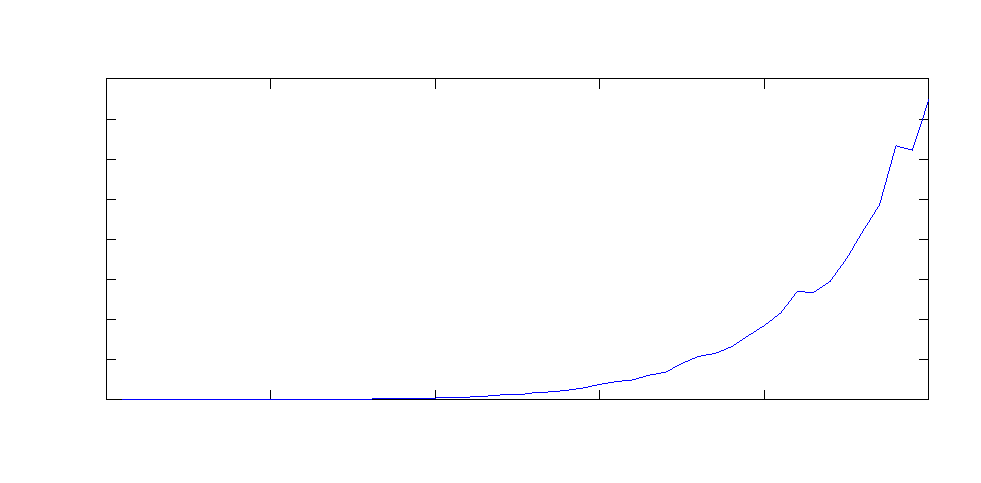
\includegraphics{exacto-random}}%
    \gplfronttext
  \end{picture}%
\endgroup

\end{figure}

Para grafos más densos el crecimiento es mucho más pronunciado y el experimento puede durar horas, mientras que para grafos más	dispersos lo opuesto ocurre y es necesario una cantidad enorme de nodos para apreciar la naturaleza exponencial del crecimiento. Escogimos la cantidad de aristas $\frac{n^2}{3}$ porque luego de probar otras cantidades en función de la cantidad de nodos, ésta resultó en un buen equilibro entre las características recién mencionadas.


\subsection{Grafos de entrenamiento}

Llamamos ``grafos de entrenamiento'' al conjunto de grafos para los que se optimizaron los parámetros de las heurísticas.



\subsubsection{Calidad de la solución}

\begin{figure}[H]
	% GNUPLOT: LaTeX picture with Postscript
\begingroup
  \makeatletter
  \providecommand\color[2][]{%
    \GenericError{(gnuplot) \space\space\space\@spaces}{%
      Package color not loaded in conjunction with
      terminal option `colourtext'%
    }{See the gnuplot documentation for explanation.%
    }{Either use 'blacktext' in gnuplot or load the package
      color.sty in LaTeX.}%
    \renewcommand\color[2][]{}%
  }%
  \providecommand\includegraphics[2][]{%
    \GenericError{(gnuplot) \space\space\space\@spaces}{%
      Package graphicx or graphics not loaded%
    }{See the gnuplot documentation for explanation.%
    }{The gnuplot epslatex terminal needs graphicx.sty or graphics.sty.}%
    \renewcommand\includegraphics[2][]{}%
  }%
  \providecommand\rotatebox[2]{#2}%
  \@ifundefined{ifGPcolor}{%
    \newif\ifGPcolor
    \GPcolorfalse
  }{}%
  \@ifundefined{ifGPblacktext}{%
    \newif\ifGPblacktext
    \GPblacktexttrue
  }{}%
  % define a \g@addto@macro without @ in the name:
  \let\gplgaddtomacro\g@addto@macro
  % define empty templates for all commands taking text:
  \gdef\gplbacktext{}%
  \gdef\gplfronttext{}%
  \makeatother
  \ifGPblacktext
    % no textcolor at all
    \def\colorrgb#1{}%
    \def\colorgray#1{}%
  \else
    % gray or color?
    \ifGPcolor
      \def\colorrgb#1{\color[rgb]{#1}}%
      \def\colorgray#1{\color[gray]{#1}}%
      \expandafter\def\csname LTw\endcsname{\color{white}}%
      \expandafter\def\csname LTb\endcsname{\color{black}}%
      \expandafter\def\csname LTa\endcsname{\color{black}}%
      \expandafter\def\csname LT0\endcsname{\color[rgb]{1,0,0}}%
      \expandafter\def\csname LT1\endcsname{\color[rgb]{0,1,0}}%
      \expandafter\def\csname LT2\endcsname{\color[rgb]{0,0,1}}%
      \expandafter\def\csname LT3\endcsname{\color[rgb]{1,0,1}}%
      \expandafter\def\csname LT4\endcsname{\color[rgb]{0,1,1}}%
      \expandafter\def\csname LT5\endcsname{\color[rgb]{1,1,0}}%
      \expandafter\def\csname LT6\endcsname{\color[rgb]{0,0,0}}%
      \expandafter\def\csname LT7\endcsname{\color[rgb]{1,0.3,0}}%
      \expandafter\def\csname LT8\endcsname{\color[rgb]{0.5,0.5,0.5}}%
    \else
      % gray
      \def\colorrgb#1{\color{black}}%
      \def\colorgray#1{\color[gray]{#1}}%
      \expandafter\def\csname LTw\endcsname{\color{white}}%
      \expandafter\def\csname LTb\endcsname{\color{black}}%
      \expandafter\def\csname LTa\endcsname{\color{black}}%
      \expandafter\def\csname LT0\endcsname{\color{black}}%
      \expandafter\def\csname LT1\endcsname{\color{black}}%
      \expandafter\def\csname LT2\endcsname{\color{black}}%
      \expandafter\def\csname LT3\endcsname{\color{black}}%
      \expandafter\def\csname LT4\endcsname{\color{black}}%
      \expandafter\def\csname LT5\endcsname{\color{black}}%
      \expandafter\def\csname LT6\endcsname{\color{black}}%
      \expandafter\def\csname LT7\endcsname{\color{black}}%
      \expandafter\def\csname LT8\endcsname{\color{black}}%
    \fi
  \fi
  \setlength{\unitlength}{0.0500bp}%
  \begin{picture}(9118.00,4320.00)%
    \gplgaddtomacro\gplbacktext{%
      \colorrgb{0.00,0.00,0.00}%
      \put(740,640){\makebox(0,0)[r]{\strut{}0}}%
      \colorrgb{0.00,0.00,0.00}%
      \put(740,1025){\makebox(0,0)[r]{\strut{}50}}%
      \colorrgb{0.00,0.00,0.00}%
      \put(740,1410){\makebox(0,0)[r]{\strut{}100}}%
      \colorrgb{0.00,0.00,0.00}%
      \put(740,1795){\makebox(0,0)[r]{\strut{}150}}%
      \colorrgb{0.00,0.00,0.00}%
      \put(740,2180){\makebox(0,0)[r]{\strut{}200}}%
      \colorrgb{0.00,0.00,0.00}%
      \put(740,2564){\makebox(0,0)[r]{\strut{}250}}%
      \colorrgb{0.00,0.00,0.00}%
      \put(740,2949){\makebox(0,0)[r]{\strut{}300}}%
      \colorrgb{0.00,0.00,0.00}%
      \put(740,3334){\makebox(0,0)[r]{\strut{}350}}%
      \colorrgb{0.00,0.00,0.00}%
      \put(740,3719){\makebox(0,0)[r]{\strut{}400}}%
      \colorrgb{0.00,0.00,0.00}%
      \put(860,440){\makebox(0,0){\strut{}0}}%
      \colorrgb{0.00,0.00,0.00}%
      \put(2834,440){\makebox(0,0){\strut{}5}}%
      \colorrgb{0.00,0.00,0.00}%
      \put(4809,440){\makebox(0,0){\strut{}10}}%
      \colorrgb{0.00,0.00,0.00}%
      \put(6783,440){\makebox(0,0){\strut{}15}}%
      \colorrgb{0.00,0.00,0.00}%
      \put(8757,440){\makebox(0,0){\strut{}20}}%
      \colorrgb{0.00,0.00,0.00}%
      \put(160,2179){\rotatebox{90}{\makebox(0,0){\strut{}Frecuencia}}}%
      \colorrgb{0.00,0.00,0.00}%
      \put(4808,140){\makebox(0,0){\strut{}Tama\~no de la frontera: diferencia respecto de la soluci\'on exacta}}%
      \csname LTb\endcsname%
      \put(4808,4019){\makebox(0,0){\strut{}Heur\'istica Golosa: calidad de las soluciones}}%
    }%
    \gplgaddtomacro\gplfronttext{%
    }%
    \gplbacktext
    \put(0,0){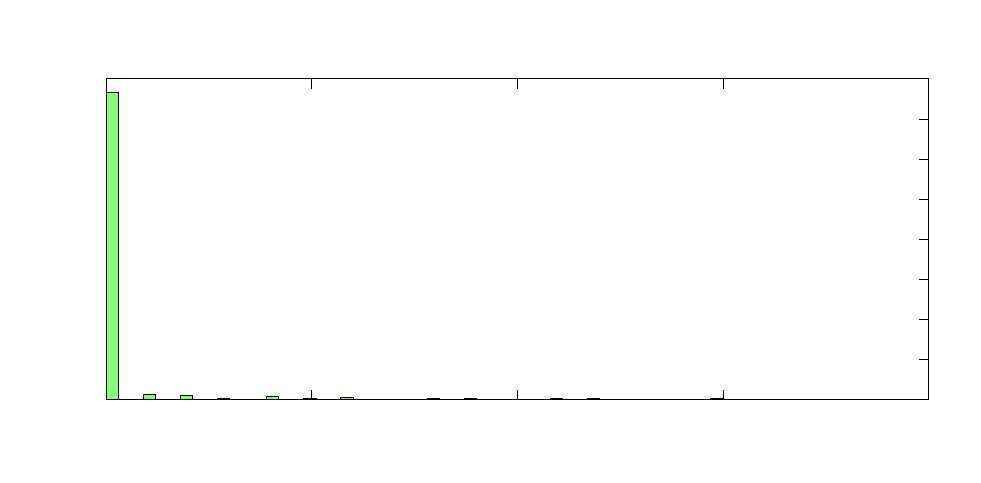
\includegraphics{golosa-calidad-entrenamiento}}%
    \gplfronttext
  \end{picture}%
\endgroup

\end{figure}

\begin{figure}[H]
	% GNUPLOT: LaTeX picture with Postscript
\begingroup
  \makeatletter
  \providecommand\color[2][]{%
    \GenericError{(gnuplot) \space\space\space\@spaces}{%
      Package color not loaded in conjunction with
      terminal option `colourtext'%
    }{See the gnuplot documentation for explanation.%
    }{Either use 'blacktext' in gnuplot or load the package
      color.sty in LaTeX.}%
    \renewcommand\color[2][]{}%
  }%
  \providecommand\includegraphics[2][]{%
    \GenericError{(gnuplot) \space\space\space\@spaces}{%
      Package graphicx or graphics not loaded%
    }{See the gnuplot documentation for explanation.%
    }{The gnuplot epslatex terminal needs graphicx.sty or graphics.sty.}%
    \renewcommand\includegraphics[2][]{}%
  }%
  \providecommand\rotatebox[2]{#2}%
  \@ifundefined{ifGPcolor}{%
    \newif\ifGPcolor
    \GPcolorfalse
  }{}%
  \@ifundefined{ifGPblacktext}{%
    \newif\ifGPblacktext
    \GPblacktexttrue
  }{}%
  % define a \g@addto@macro without @ in the name:
  \let\gplgaddtomacro\g@addto@macro
  % define empty templates for all commands taking text:
  \gdef\gplbacktext{}%
  \gdef\gplfronttext{}%
  \makeatother
  \ifGPblacktext
    % no textcolor at all
    \def\colorrgb#1{}%
    \def\colorgray#1{}%
  \else
    % gray or color?
    \ifGPcolor
      \def\colorrgb#1{\color[rgb]{#1}}%
      \def\colorgray#1{\color[gray]{#1}}%
      \expandafter\def\csname LTw\endcsname{\color{white}}%
      \expandafter\def\csname LTb\endcsname{\color{black}}%
      \expandafter\def\csname LTa\endcsname{\color{black}}%
      \expandafter\def\csname LT0\endcsname{\color[rgb]{1,0,0}}%
      \expandafter\def\csname LT1\endcsname{\color[rgb]{0,1,0}}%
      \expandafter\def\csname LT2\endcsname{\color[rgb]{0,0,1}}%
      \expandafter\def\csname LT3\endcsname{\color[rgb]{1,0,1}}%
      \expandafter\def\csname LT4\endcsname{\color[rgb]{0,1,1}}%
      \expandafter\def\csname LT5\endcsname{\color[rgb]{1,1,0}}%
      \expandafter\def\csname LT6\endcsname{\color[rgb]{0,0,0}}%
      \expandafter\def\csname LT7\endcsname{\color[rgb]{1,0.3,0}}%
      \expandafter\def\csname LT8\endcsname{\color[rgb]{0.5,0.5,0.5}}%
    \else
      % gray
      \def\colorrgb#1{\color{black}}%
      \def\colorgray#1{\color[gray]{#1}}%
      \expandafter\def\csname LTw\endcsname{\color{white}}%
      \expandafter\def\csname LTb\endcsname{\color{black}}%
      \expandafter\def\csname LTa\endcsname{\color{black}}%
      \expandafter\def\csname LT0\endcsname{\color{black}}%
      \expandafter\def\csname LT1\endcsname{\color{black}}%
      \expandafter\def\csname LT2\endcsname{\color{black}}%
      \expandafter\def\csname LT3\endcsname{\color{black}}%
      \expandafter\def\csname LT4\endcsname{\color{black}}%
      \expandafter\def\csname LT5\endcsname{\color{black}}%
      \expandafter\def\csname LT6\endcsname{\color{black}}%
      \expandafter\def\csname LT7\endcsname{\color{black}}%
      \expandafter\def\csname LT8\endcsname{\color{black}}%
    \fi
  \fi
  \setlength{\unitlength}{0.0500bp}%
  \begin{picture}(9118.00,4320.00)%
    \gplgaddtomacro\gplbacktext{%
      \colorrgb{0.00,0.00,0.00}%
      \put(740,640){\makebox(0,0)[r]{\strut{}0}}%
      \colorrgb{0.00,0.00,0.00}%
      \put(740,1153){\makebox(0,0)[r]{\strut{}50}}%
      \colorrgb{0.00,0.00,0.00}%
      \put(740,1666){\makebox(0,0)[r]{\strut{}100}}%
      \colorrgb{0.00,0.00,0.00}%
      \put(740,2180){\makebox(0,0)[r]{\strut{}150}}%
      \colorrgb{0.00,0.00,0.00}%
      \put(740,2693){\makebox(0,0)[r]{\strut{}200}}%
      \colorrgb{0.00,0.00,0.00}%
      \put(740,3206){\makebox(0,0)[r]{\strut{}250}}%
      \colorrgb{0.00,0.00,0.00}%
      \put(740,3719){\makebox(0,0)[r]{\strut{}300}}%
      \colorrgb{0.00,0.00,0.00}%
      \put(860,440){\makebox(0,0){\strut{}0}}%
      \colorrgb{0.00,0.00,0.00}%
      \put(2834,440){\makebox(0,0){\strut{}5}}%
      \colorrgb{0.00,0.00,0.00}%
      \put(4809,440){\makebox(0,0){\strut{}10}}%
      \colorrgb{0.00,0.00,0.00}%
      \put(6783,440){\makebox(0,0){\strut{}15}}%
      \colorrgb{0.00,0.00,0.00}%
      \put(8757,440){\makebox(0,0){\strut{}20}}%
      \colorrgb{0.00,0.00,0.00}%
      \put(160,2179){\rotatebox{90}{\makebox(0,0){\strut{}Frecuencia}}}%
      \colorrgb{0.00,0.00,0.00}%
      \put(4808,140){\makebox(0,0){\strut{}Tama\~no de la frontera: diferencia respecto de la soluci\'on exacta}}%
      \csname LTb\endcsname%
      \put(4808,4019){\makebox(0,0){\strut{}Heur\'istica Local: calidad de las soluciones}}%
    }%
    \gplgaddtomacro\gplfronttext{%
    }%
    \gplbacktext
    \put(0,0){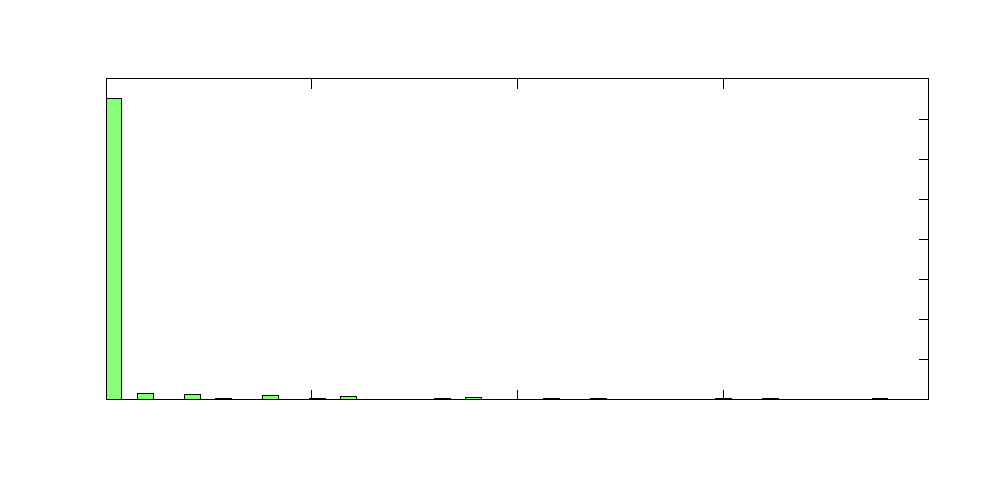
\includegraphics{local-calidad-entrenamiento}}%
    \gplfronttext
  \end{picture}%
\endgroup

\end{figure}

\begin{figure}[H]
	% GNUPLOT: LaTeX picture with Postscript
\begingroup
  \makeatletter
  \providecommand\color[2][]{%
    \GenericError{(gnuplot) \space\space\space\@spaces}{%
      Package color not loaded in conjunction with
      terminal option `colourtext'%
    }{See the gnuplot documentation for explanation.%
    }{Either use 'blacktext' in gnuplot or load the package
      color.sty in LaTeX.}%
    \renewcommand\color[2][]{}%
  }%
  \providecommand\includegraphics[2][]{%
    \GenericError{(gnuplot) \space\space\space\@spaces}{%
      Package graphicx or graphics not loaded%
    }{See the gnuplot documentation for explanation.%
    }{The gnuplot epslatex terminal needs graphicx.sty or graphics.sty.}%
    \renewcommand\includegraphics[2][]{}%
  }%
  \providecommand\rotatebox[2]{#2}%
  \@ifundefined{ifGPcolor}{%
    \newif\ifGPcolor
    \GPcolorfalse
  }{}%
  \@ifundefined{ifGPblacktext}{%
    \newif\ifGPblacktext
    \GPblacktexttrue
  }{}%
  % define a \g@addto@macro without @ in the name:
  \let\gplgaddtomacro\g@addto@macro
  % define empty templates for all commands taking text:
  \gdef\gplbacktext{}%
  \gdef\gplfronttext{}%
  \makeatother
  \ifGPblacktext
    % no textcolor at all
    \def\colorrgb#1{}%
    \def\colorgray#1{}%
  \else
    % gray or color?
    \ifGPcolor
      \def\colorrgb#1{\color[rgb]{#1}}%
      \def\colorgray#1{\color[gray]{#1}}%
      \expandafter\def\csname LTw\endcsname{\color{white}}%
      \expandafter\def\csname LTb\endcsname{\color{black}}%
      \expandafter\def\csname LTa\endcsname{\color{black}}%
      \expandafter\def\csname LT0\endcsname{\color[rgb]{1,0,0}}%
      \expandafter\def\csname LT1\endcsname{\color[rgb]{0,1,0}}%
      \expandafter\def\csname LT2\endcsname{\color[rgb]{0,0,1}}%
      \expandafter\def\csname LT3\endcsname{\color[rgb]{1,0,1}}%
      \expandafter\def\csname LT4\endcsname{\color[rgb]{0,1,1}}%
      \expandafter\def\csname LT5\endcsname{\color[rgb]{1,1,0}}%
      \expandafter\def\csname LT6\endcsname{\color[rgb]{0,0,0}}%
      \expandafter\def\csname LT7\endcsname{\color[rgb]{1,0.3,0}}%
      \expandafter\def\csname LT8\endcsname{\color[rgb]{0.5,0.5,0.5}}%
    \else
      % gray
      \def\colorrgb#1{\color{black}}%
      \def\colorgray#1{\color[gray]{#1}}%
      \expandafter\def\csname LTw\endcsname{\color{white}}%
      \expandafter\def\csname LTb\endcsname{\color{black}}%
      \expandafter\def\csname LTa\endcsname{\color{black}}%
      \expandafter\def\csname LT0\endcsname{\color{black}}%
      \expandafter\def\csname LT1\endcsname{\color{black}}%
      \expandafter\def\csname LT2\endcsname{\color{black}}%
      \expandafter\def\csname LT3\endcsname{\color{black}}%
      \expandafter\def\csname LT4\endcsname{\color{black}}%
      \expandafter\def\csname LT5\endcsname{\color{black}}%
      \expandafter\def\csname LT6\endcsname{\color{black}}%
      \expandafter\def\csname LT7\endcsname{\color{black}}%
      \expandafter\def\csname LT8\endcsname{\color{black}}%
    \fi
  \fi
  \setlength{\unitlength}{0.0500bp}%
  \begin{picture}(9118.00,4320.00)%
    \gplgaddtomacro\gplbacktext{%
      \colorrgb{0.00,0.00,0.00}%
      \put(740,640){\makebox(0,0)[r]{\strut{}0}}%
      \colorrgb{0.00,0.00,0.00}%
      \put(740,1025){\makebox(0,0)[r]{\strut{}50}}%
      \colorrgb{0.00,0.00,0.00}%
      \put(740,1410){\makebox(0,0)[r]{\strut{}100}}%
      \colorrgb{0.00,0.00,0.00}%
      \put(740,1795){\makebox(0,0)[r]{\strut{}150}}%
      \colorrgb{0.00,0.00,0.00}%
      \put(740,2180){\makebox(0,0)[r]{\strut{}200}}%
      \colorrgb{0.00,0.00,0.00}%
      \put(740,2564){\makebox(0,0)[r]{\strut{}250}}%
      \colorrgb{0.00,0.00,0.00}%
      \put(740,2949){\makebox(0,0)[r]{\strut{}300}}%
      \colorrgb{0.00,0.00,0.00}%
      \put(740,3334){\makebox(0,0)[r]{\strut{}350}}%
      \colorrgb{0.00,0.00,0.00}%
      \put(740,3719){\makebox(0,0)[r]{\strut{}400}}%
      \colorrgb{0.00,0.00,0.00}%
      \put(860,440){\makebox(0,0){\strut{}0}}%
      \colorrgb{0.00,0.00,0.00}%
      \put(2176,440){\makebox(0,0){\strut{}1}}%
      \colorrgb{0.00,0.00,0.00}%
      \put(3492,440){\makebox(0,0){\strut{}2}}%
      \colorrgb{0.00,0.00,0.00}%
      \put(4809,440){\makebox(0,0){\strut{}3}}%
      \colorrgb{0.00,0.00,0.00}%
      \put(6125,440){\makebox(0,0){\strut{}4}}%
      \colorrgb{0.00,0.00,0.00}%
      \put(7441,440){\makebox(0,0){\strut{}5}}%
      \colorrgb{0.00,0.00,0.00}%
      \put(8757,440){\makebox(0,0){\strut{}6}}%
      \colorrgb{0.00,0.00,0.00}%
      \put(160,2179){\rotatebox{90}{\makebox(0,0){\strut{}Frecuencia}}}%
      \colorrgb{0.00,0.00,0.00}%
      \put(4808,140){\makebox(0,0){\strut{}Tama\~no de la frontera: diferencia respecto de la soluci\'on exacta}}%
      \csname LTb\endcsname%
      \put(4808,4019){\makebox(0,0){\strut{}Heur\'istica Tab\'u: calidad de las soluciones}}%
    }%
    \gplgaddtomacro\gplfronttext{%
    }%
    \gplbacktext
    \put(0,0){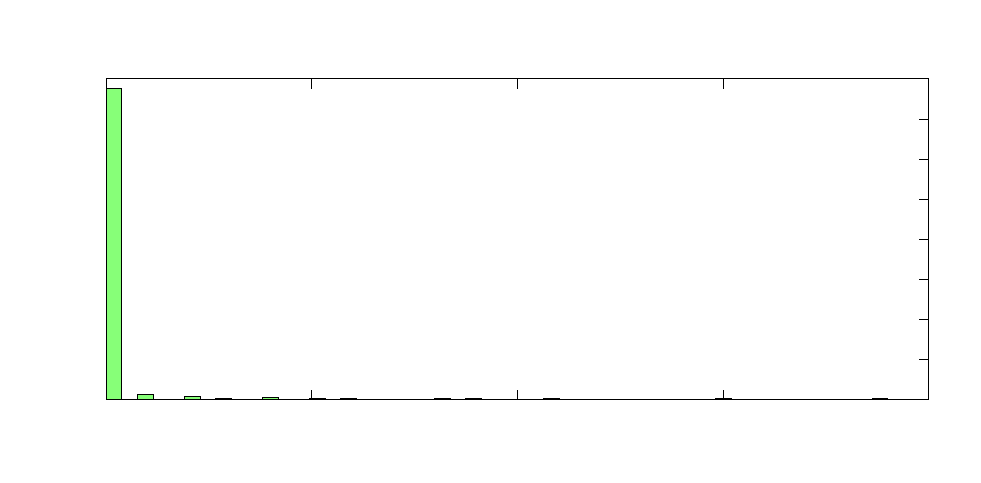
\includegraphics{tabu-calidad-entrenamiento}}%
    \gplfronttext
  \end{picture}%
\endgroup

\end{figure}


\subsubsection{Tiempo de ejecución}

\begin{figure}[H]
	% GNUPLOT: LaTeX picture with Postscript
\begingroup
  \makeatletter
  \providecommand\color[2][]{%
    \GenericError{(gnuplot) \space\space\space\@spaces}{%
      Package color not loaded in conjunction with
      terminal option `colourtext'%
    }{See the gnuplot documentation for explanation.%
    }{Either use 'blacktext' in gnuplot or load the package
      color.sty in LaTeX.}%
    \renewcommand\color[2][]{}%
  }%
  \providecommand\includegraphics[2][]{%
    \GenericError{(gnuplot) \space\space\space\@spaces}{%
      Package graphicx or graphics not loaded%
    }{See the gnuplot documentation for explanation.%
    }{The gnuplot epslatex terminal needs graphicx.sty or graphics.sty.}%
    \renewcommand\includegraphics[2][]{}%
  }%
  \providecommand\rotatebox[2]{#2}%
  \@ifundefined{ifGPcolor}{%
    \newif\ifGPcolor
    \GPcolorfalse
  }{}%
  \@ifundefined{ifGPblacktext}{%
    \newif\ifGPblacktext
    \GPblacktexttrue
  }{}%
  % define a \g@addto@macro without @ in the name:
  \let\gplgaddtomacro\g@addto@macro
  % define empty templates for all commands taking text:
  \gdef\gplbacktext{}%
  \gdef\gplfronttext{}%
  \makeatother
  \ifGPblacktext
    % no textcolor at all
    \def\colorrgb#1{}%
    \def\colorgray#1{}%
  \else
    % gray or color?
    \ifGPcolor
      \def\colorrgb#1{\color[rgb]{#1}}%
      \def\colorgray#1{\color[gray]{#1}}%
      \expandafter\def\csname LTw\endcsname{\color{white}}%
      \expandafter\def\csname LTb\endcsname{\color{black}}%
      \expandafter\def\csname LTa\endcsname{\color{black}}%
      \expandafter\def\csname LT0\endcsname{\color[rgb]{1,0,0}}%
      \expandafter\def\csname LT1\endcsname{\color[rgb]{0,1,0}}%
      \expandafter\def\csname LT2\endcsname{\color[rgb]{0,0,1}}%
      \expandafter\def\csname LT3\endcsname{\color[rgb]{1,0,1}}%
      \expandafter\def\csname LT4\endcsname{\color[rgb]{0,1,1}}%
      \expandafter\def\csname LT5\endcsname{\color[rgb]{1,1,0}}%
      \expandafter\def\csname LT6\endcsname{\color[rgb]{0,0,0}}%
      \expandafter\def\csname LT7\endcsname{\color[rgb]{1,0.3,0}}%
      \expandafter\def\csname LT8\endcsname{\color[rgb]{0.5,0.5,0.5}}%
    \else
      % gray
      \def\colorrgb#1{\color{black}}%
      \def\colorgray#1{\color[gray]{#1}}%
      \expandafter\def\csname LTw\endcsname{\color{white}}%
      \expandafter\def\csname LTb\endcsname{\color{black}}%
      \expandafter\def\csname LTa\endcsname{\color{black}}%
      \expandafter\def\csname LT0\endcsname{\color{black}}%
      \expandafter\def\csname LT1\endcsname{\color{black}}%
      \expandafter\def\csname LT2\endcsname{\color{black}}%
      \expandafter\def\csname LT3\endcsname{\color{black}}%
      \expandafter\def\csname LT4\endcsname{\color{black}}%
      \expandafter\def\csname LT5\endcsname{\color{black}}%
      \expandafter\def\csname LT6\endcsname{\color{black}}%
      \expandafter\def\csname LT7\endcsname{\color{black}}%
      \expandafter\def\csname LT8\endcsname{\color{black}}%
    \fi
  \fi
  \setlength{\unitlength}{0.0500bp}%
  \begin{picture}(9118.00,4320.00)%
    \gplgaddtomacro\gplbacktext{%
      \colorrgb{0.00,0.00,0.00}%
      \put(740,640){\makebox(0,0)[r]{\strut{}0}}%
      \colorrgb{0.00,0.00,0.00}%
      \put(740,1256){\makebox(0,0)[r]{\strut{}20}}%
      \colorrgb{0.00,0.00,0.00}%
      \put(740,1872){\makebox(0,0)[r]{\strut{}40}}%
      \colorrgb{0.00,0.00,0.00}%
      \put(740,2487){\makebox(0,0)[r]{\strut{}60}}%
      \colorrgb{0.00,0.00,0.00}%
      \put(740,3103){\makebox(0,0)[r]{\strut{}80}}%
      \colorrgb{0.00,0.00,0.00}%
      \put(740,3719){\makebox(0,0)[r]{\strut{}100}}%
      \colorrgb{0.00,0.00,0.00}%
      \put(860,440){\makebox(0,0){\strut{}0}}%
      \colorrgb{0.00,0.00,0.00}%
      \put(1988,440){\makebox(0,0){\strut{}0.05}}%
      \colorrgb{0.00,0.00,0.00}%
      \put(3116,440){\makebox(0,0){\strut{}0.1}}%
      \colorrgb{0.00,0.00,0.00}%
      \put(4244,440){\makebox(0,0){\strut{}0.15}}%
      \colorrgb{0.00,0.00,0.00}%
      \put(5373,440){\makebox(0,0){\strut{}0.2}}%
      \colorrgb{0.00,0.00,0.00}%
      \put(6501,440){\makebox(0,0){\strut{}0.25}}%
      \colorrgb{0.00,0.00,0.00}%
      \put(7629,440){\makebox(0,0){\strut{}0.3}}%
      \colorrgb{0.00,0.00,0.00}%
      \put(8757,440){\makebox(0,0){\strut{}0.35}}%
      \colorrgb{0.00,0.00,0.00}%
      \put(160,2179){\rotatebox{90}{\makebox(0,0){\strut{}Frecuencia}}}%
      \colorrgb{0.00,0.00,0.00}%
      \put(4808,140){\makebox(0,0){\strut{}Tiempo de ejecuci\'on (milisegundos)}}%
      \csname LTb\endcsname%
      \put(4808,4019){\makebox(0,0){\strut{}Heur\'istica Golosa: tiempo de ejecuci\'on}}%
    }%
    \gplgaddtomacro\gplfronttext{%
    }%
    \gplbacktext
    \put(0,0){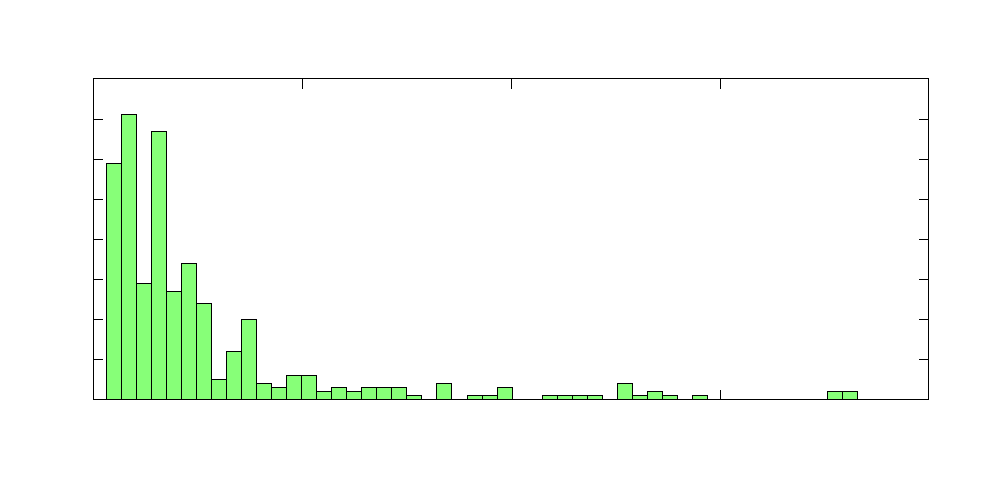
\includegraphics{golosa-tiempo-entrenamiento}}%
    \gplfronttext
  \end{picture}%
\endgroup

\end{figure}

\begin{figure}[H]
	% GNUPLOT: LaTeX picture with Postscript
\begingroup
  \makeatletter
  \providecommand\color[2][]{%
    \GenericError{(gnuplot) \space\space\space\@spaces}{%
      Package color not loaded in conjunction with
      terminal option `colourtext'%
    }{See the gnuplot documentation for explanation.%
    }{Either use 'blacktext' in gnuplot or load the package
      color.sty in LaTeX.}%
    \renewcommand\color[2][]{}%
  }%
  \providecommand\includegraphics[2][]{%
    \GenericError{(gnuplot) \space\space\space\@spaces}{%
      Package graphicx or graphics not loaded%
    }{See the gnuplot documentation for explanation.%
    }{The gnuplot epslatex terminal needs graphicx.sty or graphics.sty.}%
    \renewcommand\includegraphics[2][]{}%
  }%
  \providecommand\rotatebox[2]{#2}%
  \@ifundefined{ifGPcolor}{%
    \newif\ifGPcolor
    \GPcolorfalse
  }{}%
  \@ifundefined{ifGPblacktext}{%
    \newif\ifGPblacktext
    \GPblacktexttrue
  }{}%
  % define a \g@addto@macro without @ in the name:
  \let\gplgaddtomacro\g@addto@macro
  % define empty templates for all commands taking text:
  \gdef\gplbacktext{}%
  \gdef\gplfronttext{}%
  \makeatother
  \ifGPblacktext
    % no textcolor at all
    \def\colorrgb#1{}%
    \def\colorgray#1{}%
  \else
    % gray or color?
    \ifGPcolor
      \def\colorrgb#1{\color[rgb]{#1}}%
      \def\colorgray#1{\color[gray]{#1}}%
      \expandafter\def\csname LTw\endcsname{\color{white}}%
      \expandafter\def\csname LTb\endcsname{\color{black}}%
      \expandafter\def\csname LTa\endcsname{\color{black}}%
      \expandafter\def\csname LT0\endcsname{\color[rgb]{1,0,0}}%
      \expandafter\def\csname LT1\endcsname{\color[rgb]{0,1,0}}%
      \expandafter\def\csname LT2\endcsname{\color[rgb]{0,0,1}}%
      \expandafter\def\csname LT3\endcsname{\color[rgb]{1,0,1}}%
      \expandafter\def\csname LT4\endcsname{\color[rgb]{0,1,1}}%
      \expandafter\def\csname LT5\endcsname{\color[rgb]{1,1,0}}%
      \expandafter\def\csname LT6\endcsname{\color[rgb]{0,0,0}}%
      \expandafter\def\csname LT7\endcsname{\color[rgb]{1,0.3,0}}%
      \expandafter\def\csname LT8\endcsname{\color[rgb]{0.5,0.5,0.5}}%
    \else
      % gray
      \def\colorrgb#1{\color{black}}%
      \def\colorgray#1{\color[gray]{#1}}%
      \expandafter\def\csname LTw\endcsname{\color{white}}%
      \expandafter\def\csname LTb\endcsname{\color{black}}%
      \expandafter\def\csname LTa\endcsname{\color{black}}%
      \expandafter\def\csname LT0\endcsname{\color{black}}%
      \expandafter\def\csname LT1\endcsname{\color{black}}%
      \expandafter\def\csname LT2\endcsname{\color{black}}%
      \expandafter\def\csname LT3\endcsname{\color{black}}%
      \expandafter\def\csname LT4\endcsname{\color{black}}%
      \expandafter\def\csname LT5\endcsname{\color{black}}%
      \expandafter\def\csname LT6\endcsname{\color{black}}%
      \expandafter\def\csname LT7\endcsname{\color{black}}%
      \expandafter\def\csname LT8\endcsname{\color{black}}%
    \fi
  \fi
  \setlength{\unitlength}{0.0500bp}%
  \begin{picture}(9118.00,4320.00)%
    \gplgaddtomacro\gplbacktext{%
      \colorrgb{0.00,0.00,0.00}%
      \put(620,640){\makebox(0,0)[r]{\strut{}0}}%
      \colorrgb{0.00,0.00,0.00}%
      \put(620,1080){\makebox(0,0)[r]{\strut{}10}}%
      \colorrgb{0.00,0.00,0.00}%
      \put(620,1520){\makebox(0,0)[r]{\strut{}20}}%
      \colorrgb{0.00,0.00,0.00}%
      \put(620,1960){\makebox(0,0)[r]{\strut{}30}}%
      \colorrgb{0.00,0.00,0.00}%
      \put(620,2399){\makebox(0,0)[r]{\strut{}40}}%
      \colorrgb{0.00,0.00,0.00}%
      \put(620,2839){\makebox(0,0)[r]{\strut{}50}}%
      \colorrgb{0.00,0.00,0.00}%
      \put(620,3279){\makebox(0,0)[r]{\strut{}60}}%
      \colorrgb{0.00,0.00,0.00}%
      \put(620,3719){\makebox(0,0)[r]{\strut{}70}}%
      \colorrgb{0.00,0.00,0.00}%
      \put(740,440){\makebox(0,0){\strut{}0}}%
      \colorrgb{0.00,0.00,0.00}%
      \put(1885,440){\makebox(0,0){\strut{}0.1}}%
      \colorrgb{0.00,0.00,0.00}%
      \put(3031,440){\makebox(0,0){\strut{}0.2}}%
      \colorrgb{0.00,0.00,0.00}%
      \put(4176,440){\makebox(0,0){\strut{}0.3}}%
      \colorrgb{0.00,0.00,0.00}%
      \put(5321,440){\makebox(0,0){\strut{}0.4}}%
      \colorrgb{0.00,0.00,0.00}%
      \put(6466,440){\makebox(0,0){\strut{}0.5}}%
      \colorrgb{0.00,0.00,0.00}%
      \put(7612,440){\makebox(0,0){\strut{}0.6}}%
      \colorrgb{0.00,0.00,0.00}%
      \put(8757,440){\makebox(0,0){\strut{}0.7}}%
      \colorrgb{0.00,0.00,0.00}%
      \put(160,2179){\rotatebox{90}{\makebox(0,0){\strut{}Frecuencia}}}%
      \colorrgb{0.00,0.00,0.00}%
      \put(4748,140){\makebox(0,0){\strut{}Tiempo de ejecuci\'on (milisegundos)}}%
      \csname LTb\endcsname%
      \put(4748,4019){\makebox(0,0){\strut{}Heur\'istica Local: tiempo de ejecuci\'on}}%
    }%
    \gplgaddtomacro\gplfronttext{%
    }%
    \gplbacktext
    \put(0,0){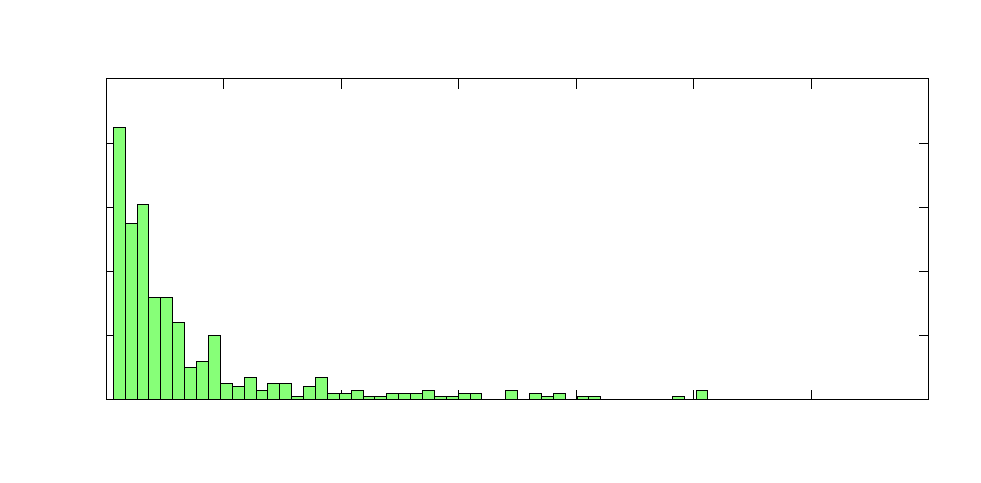
\includegraphics{local-tiempo-entrenamiento}}%
    \gplfronttext
  \end{picture}%
\endgroup

\end{figure}

\begin{figure}[H]
	% GNUPLOT: LaTeX picture with Postscript
\begingroup
  \makeatletter
  \providecommand\color[2][]{%
    \GenericError{(gnuplot) \space\space\space\@spaces}{%
      Package color not loaded in conjunction with
      terminal option `colourtext'%
    }{See the gnuplot documentation for explanation.%
    }{Either use 'blacktext' in gnuplot or load the package
      color.sty in LaTeX.}%
    \renewcommand\color[2][]{}%
  }%
  \providecommand\includegraphics[2][]{%
    \GenericError{(gnuplot) \space\space\space\@spaces}{%
      Package graphicx or graphics not loaded%
    }{See the gnuplot documentation for explanation.%
    }{The gnuplot epslatex terminal needs graphicx.sty or graphics.sty.}%
    \renewcommand\includegraphics[2][]{}%
  }%
  \providecommand\rotatebox[2]{#2}%
  \@ifundefined{ifGPcolor}{%
    \newif\ifGPcolor
    \GPcolorfalse
  }{}%
  \@ifundefined{ifGPblacktext}{%
    \newif\ifGPblacktext
    \GPblacktexttrue
  }{}%
  % define a \g@addto@macro without @ in the name:
  \let\gplgaddtomacro\g@addto@macro
  % define empty templates for all commands taking text:
  \gdef\gplbacktext{}%
  \gdef\gplfronttext{}%
  \makeatother
  \ifGPblacktext
    % no textcolor at all
    \def\colorrgb#1{}%
    \def\colorgray#1{}%
  \else
    % gray or color?
    \ifGPcolor
      \def\colorrgb#1{\color[rgb]{#1}}%
      \def\colorgray#1{\color[gray]{#1}}%
      \expandafter\def\csname LTw\endcsname{\color{white}}%
      \expandafter\def\csname LTb\endcsname{\color{black}}%
      \expandafter\def\csname LTa\endcsname{\color{black}}%
      \expandafter\def\csname LT0\endcsname{\color[rgb]{1,0,0}}%
      \expandafter\def\csname LT1\endcsname{\color[rgb]{0,1,0}}%
      \expandafter\def\csname LT2\endcsname{\color[rgb]{0,0,1}}%
      \expandafter\def\csname LT3\endcsname{\color[rgb]{1,0,1}}%
      \expandafter\def\csname LT4\endcsname{\color[rgb]{0,1,1}}%
      \expandafter\def\csname LT5\endcsname{\color[rgb]{1,1,0}}%
      \expandafter\def\csname LT6\endcsname{\color[rgb]{0,0,0}}%
      \expandafter\def\csname LT7\endcsname{\color[rgb]{1,0.3,0}}%
      \expandafter\def\csname LT8\endcsname{\color[rgb]{0.5,0.5,0.5}}%
    \else
      % gray
      \def\colorrgb#1{\color{black}}%
      \def\colorgray#1{\color[gray]{#1}}%
      \expandafter\def\csname LTw\endcsname{\color{white}}%
      \expandafter\def\csname LTb\endcsname{\color{black}}%
      \expandafter\def\csname LTa\endcsname{\color{black}}%
      \expandafter\def\csname LT0\endcsname{\color{black}}%
      \expandafter\def\csname LT1\endcsname{\color{black}}%
      \expandafter\def\csname LT2\endcsname{\color{black}}%
      \expandafter\def\csname LT3\endcsname{\color{black}}%
      \expandafter\def\csname LT4\endcsname{\color{black}}%
      \expandafter\def\csname LT5\endcsname{\color{black}}%
      \expandafter\def\csname LT6\endcsname{\color{black}}%
      \expandafter\def\csname LT7\endcsname{\color{black}}%
      \expandafter\def\csname LT8\endcsname{\color{black}}%
    \fi
  \fi
  \setlength{\unitlength}{0.0500bp}%
  \begin{picture}(9118.00,4320.00)%
    \gplgaddtomacro\gplbacktext{%
      \colorrgb{0.00,0.00,0.00}%
      \put(740,640){\makebox(0,0)[r]{\strut{}0}}%
      \colorrgb{0.00,0.00,0.00}%
      \put(740,1256){\makebox(0,0)[r]{\strut{}20}}%
      \colorrgb{0.00,0.00,0.00}%
      \put(740,1872){\makebox(0,0)[r]{\strut{}40}}%
      \colorrgb{0.00,0.00,0.00}%
      \put(740,2487){\makebox(0,0)[r]{\strut{}60}}%
      \colorrgb{0.00,0.00,0.00}%
      \put(740,3103){\makebox(0,0)[r]{\strut{}80}}%
      \colorrgb{0.00,0.00,0.00}%
      \put(740,3719){\makebox(0,0)[r]{\strut{}100}}%
      \colorrgb{0.00,0.00,0.00}%
      \put(860,440){\makebox(0,0){\strut{}0}}%
      \colorrgb{0.00,0.00,0.00}%
      \put(2439,440){\makebox(0,0){\strut{}2}}%
      \colorrgb{0.00,0.00,0.00}%
      \put(4019,440){\makebox(0,0){\strut{}4}}%
      \colorrgb{0.00,0.00,0.00}%
      \put(5598,440){\makebox(0,0){\strut{}6}}%
      \colorrgb{0.00,0.00,0.00}%
      \put(7178,440){\makebox(0,0){\strut{}8}}%
      \colorrgb{0.00,0.00,0.00}%
      \put(8757,440){\makebox(0,0){\strut{}10}}%
      \colorrgb{0.00,0.00,0.00}%
      \put(160,2179){\rotatebox{90}{\makebox(0,0){\strut{}Frecuencia}}}%
      \colorrgb{0.00,0.00,0.00}%
      \put(4808,140){\makebox(0,0){\strut{}Tiempo de ejecuci\'on (milisegundos)}}%
      \csname LTb\endcsname%
      \put(4808,4019){\makebox(0,0){\strut{}Heur\'istica Tab\'u: tiempo de ejecuci\'on}}%
    }%
    \gplgaddtomacro\gplfronttext{%
    }%
    \gplbacktext
    \put(0,0){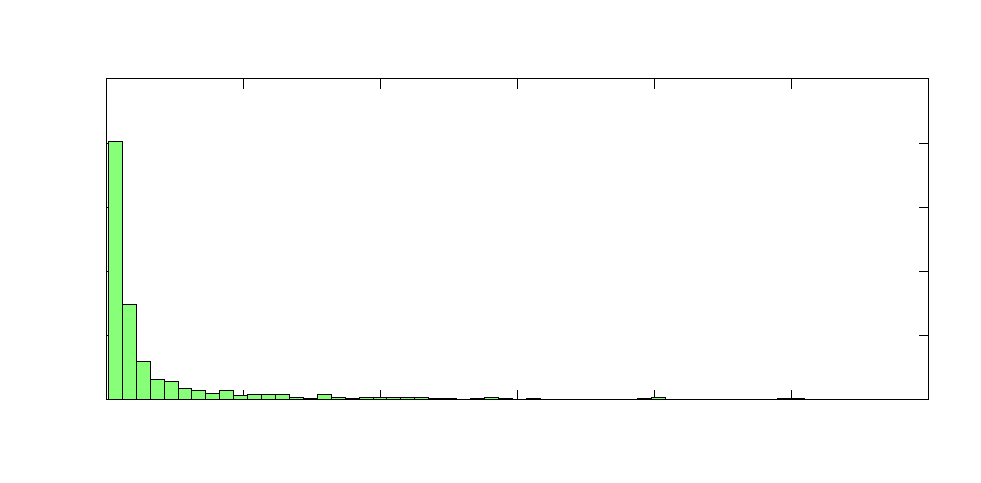
\includegraphics{tabu-tiempo-entrenamiento}}%
    \gplfronttext
  \end{picture}%
\endgroup

\end{figure}


\subsection{Grafos de testing}


\subsubsection{Calidad de la solución}

\begin{figure}[H]
	% GNUPLOT: LaTeX picture with Postscript
\begingroup
  \makeatletter
  \providecommand\color[2][]{%
    \GenericError{(gnuplot) \space\space\space\@spaces}{%
      Package color not loaded in conjunction with
      terminal option `colourtext'%
    }{See the gnuplot documentation for explanation.%
    }{Either use 'blacktext' in gnuplot or load the package
      color.sty in LaTeX.}%
    \renewcommand\color[2][]{}%
  }%
  \providecommand\includegraphics[2][]{%
    \GenericError{(gnuplot) \space\space\space\@spaces}{%
      Package graphicx or graphics not loaded%
    }{See the gnuplot documentation for explanation.%
    }{The gnuplot epslatex terminal needs graphicx.sty or graphics.sty.}%
    \renewcommand\includegraphics[2][]{}%
  }%
  \providecommand\rotatebox[2]{#2}%
  \@ifundefined{ifGPcolor}{%
    \newif\ifGPcolor
    \GPcolorfalse
  }{}%
  \@ifundefined{ifGPblacktext}{%
    \newif\ifGPblacktext
    \GPblacktexttrue
  }{}%
  % define a \g@addto@macro without @ in the name:
  \let\gplgaddtomacro\g@addto@macro
  % define empty templates for all commands taking text:
  \gdef\gplbacktext{}%
  \gdef\gplfronttext{}%
  \makeatother
  \ifGPblacktext
    % no textcolor at all
    \def\colorrgb#1{}%
    \def\colorgray#1{}%
  \else
    % gray or color?
    \ifGPcolor
      \def\colorrgb#1{\color[rgb]{#1}}%
      \def\colorgray#1{\color[gray]{#1}}%
      \expandafter\def\csname LTw\endcsname{\color{white}}%
      \expandafter\def\csname LTb\endcsname{\color{black}}%
      \expandafter\def\csname LTa\endcsname{\color{black}}%
      \expandafter\def\csname LT0\endcsname{\color[rgb]{1,0,0}}%
      \expandafter\def\csname LT1\endcsname{\color[rgb]{0,1,0}}%
      \expandafter\def\csname LT2\endcsname{\color[rgb]{0,0,1}}%
      \expandafter\def\csname LT3\endcsname{\color[rgb]{1,0,1}}%
      \expandafter\def\csname LT4\endcsname{\color[rgb]{0,1,1}}%
      \expandafter\def\csname LT5\endcsname{\color[rgb]{1,1,0}}%
      \expandafter\def\csname LT6\endcsname{\color[rgb]{0,0,0}}%
      \expandafter\def\csname LT7\endcsname{\color[rgb]{1,0.3,0}}%
      \expandafter\def\csname LT8\endcsname{\color[rgb]{0.5,0.5,0.5}}%
    \else
      % gray
      \def\colorrgb#1{\color{black}}%
      \def\colorgray#1{\color[gray]{#1}}%
      \expandafter\def\csname LTw\endcsname{\color{white}}%
      \expandafter\def\csname LTb\endcsname{\color{black}}%
      \expandafter\def\csname LTa\endcsname{\color{black}}%
      \expandafter\def\csname LT0\endcsname{\color{black}}%
      \expandafter\def\csname LT1\endcsname{\color{black}}%
      \expandafter\def\csname LT2\endcsname{\color{black}}%
      \expandafter\def\csname LT3\endcsname{\color{black}}%
      \expandafter\def\csname LT4\endcsname{\color{black}}%
      \expandafter\def\csname LT5\endcsname{\color{black}}%
      \expandafter\def\csname LT6\endcsname{\color{black}}%
      \expandafter\def\csname LT7\endcsname{\color{black}}%
      \expandafter\def\csname LT8\endcsname{\color{black}}%
    \fi
  \fi
  \setlength{\unitlength}{0.0500bp}%
  \begin{picture}(9118.00,4320.00)%
    \gplgaddtomacro\gplbacktext{%
      \colorrgb{0.00,0.00,0.00}%
      \put(620,640){\makebox(0,0)[r]{\strut{}0}}%
      \colorrgb{0.00,0.00,0.00}%
      \put(620,1025){\makebox(0,0)[r]{\strut{}5}}%
      \colorrgb{0.00,0.00,0.00}%
      \put(620,1410){\makebox(0,0)[r]{\strut{}10}}%
      \colorrgb{0.00,0.00,0.00}%
      \put(620,1795){\makebox(0,0)[r]{\strut{}15}}%
      \colorrgb{0.00,0.00,0.00}%
      \put(620,2180){\makebox(0,0)[r]{\strut{}20}}%
      \colorrgb{0.00,0.00,0.00}%
      \put(620,2564){\makebox(0,0)[r]{\strut{}25}}%
      \colorrgb{0.00,0.00,0.00}%
      \put(620,2949){\makebox(0,0)[r]{\strut{}30}}%
      \colorrgb{0.00,0.00,0.00}%
      \put(620,3334){\makebox(0,0)[r]{\strut{}35}}%
      \colorrgb{0.00,0.00,0.00}%
      \put(620,3719){\makebox(0,0)[r]{\strut{}40}}%
      \colorrgb{0.00,0.00,0.00}%
      \put(740,440){\makebox(0,0){\strut{}-1}}%
      \colorrgb{0.00,0.00,0.00}%
      \put(2744,440){\makebox(0,0){\strut{}-0.5}}%
      \colorrgb{0.00,0.00,0.00}%
      \put(4749,440){\makebox(0,0){\strut{}0}}%
      \colorrgb{0.00,0.00,0.00}%
      \put(6753,440){\makebox(0,0){\strut{}0.5}}%
      \colorrgb{0.00,0.00,0.00}%
      \put(8757,440){\makebox(0,0){\strut{}1}}%
      \colorrgb{0.00,0.00,0.00}%
      \put(160,2179){\rotatebox{90}{\makebox(0,0){\strut{}Frecuencia}}}%
      \colorrgb{0.00,0.00,0.00}%
      \put(4748,140){\makebox(0,0){\strut{}Tama\~no de la frontera: diferencia respecto de la soluci\'on exacta}}%
      \csname LTb\endcsname%
      \put(4748,4019){\makebox(0,0){\strut{}Heur\'istica Golosa: calidad de las soluciones}}%
    }%
    \gplgaddtomacro\gplfronttext{%
    }%
    \gplbacktext
    \put(0,0){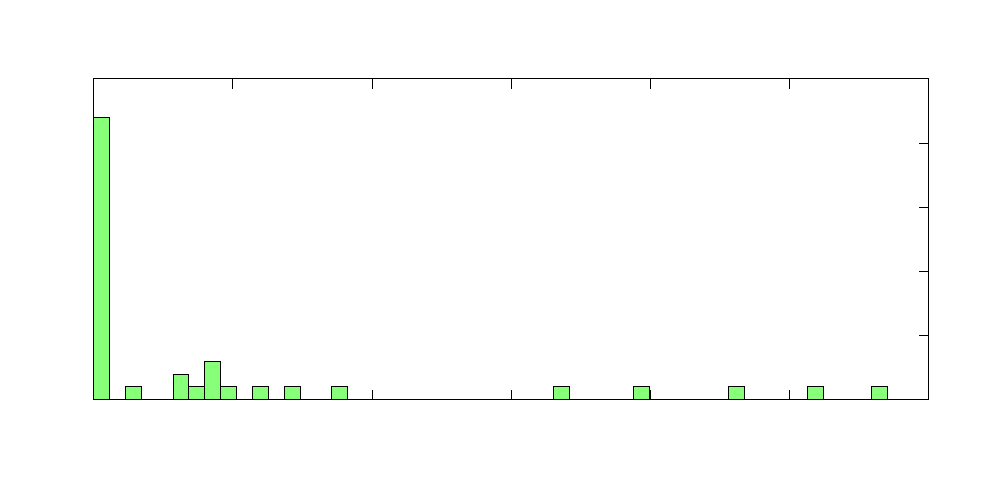
\includegraphics{golosa-calidad-testing}}%
    \gplfronttext
  \end{picture}%
\endgroup

\end{figure}

\begin{figure}[H]
	% GNUPLOT: LaTeX picture with Postscript
\begingroup
  \makeatletter
  \providecommand\color[2][]{%
    \GenericError{(gnuplot) \space\space\space\@spaces}{%
      Package color not loaded in conjunction with
      terminal option `colourtext'%
    }{See the gnuplot documentation for explanation.%
    }{Either use 'blacktext' in gnuplot or load the package
      color.sty in LaTeX.}%
    \renewcommand\color[2][]{}%
  }%
  \providecommand\includegraphics[2][]{%
    \GenericError{(gnuplot) \space\space\space\@spaces}{%
      Package graphicx or graphics not loaded%
    }{See the gnuplot documentation for explanation.%
    }{The gnuplot epslatex terminal needs graphicx.sty or graphics.sty.}%
    \renewcommand\includegraphics[2][]{}%
  }%
  \providecommand\rotatebox[2]{#2}%
  \@ifundefined{ifGPcolor}{%
    \newif\ifGPcolor
    \GPcolorfalse
  }{}%
  \@ifundefined{ifGPblacktext}{%
    \newif\ifGPblacktext
    \GPblacktexttrue
  }{}%
  % define a \g@addto@macro without @ in the name:
  \let\gplgaddtomacro\g@addto@macro
  % define empty templates for all commands taking text:
  \gdef\gplbacktext{}%
  \gdef\gplfronttext{}%
  \makeatother
  \ifGPblacktext
    % no textcolor at all
    \def\colorrgb#1{}%
    \def\colorgray#1{}%
  \else
    % gray or color?
    \ifGPcolor
      \def\colorrgb#1{\color[rgb]{#1}}%
      \def\colorgray#1{\color[gray]{#1}}%
      \expandafter\def\csname LTw\endcsname{\color{white}}%
      \expandafter\def\csname LTb\endcsname{\color{black}}%
      \expandafter\def\csname LTa\endcsname{\color{black}}%
      \expandafter\def\csname LT0\endcsname{\color[rgb]{1,0,0}}%
      \expandafter\def\csname LT1\endcsname{\color[rgb]{0,1,0}}%
      \expandafter\def\csname LT2\endcsname{\color[rgb]{0,0,1}}%
      \expandafter\def\csname LT3\endcsname{\color[rgb]{1,0,1}}%
      \expandafter\def\csname LT4\endcsname{\color[rgb]{0,1,1}}%
      \expandafter\def\csname LT5\endcsname{\color[rgb]{1,1,0}}%
      \expandafter\def\csname LT6\endcsname{\color[rgb]{0,0,0}}%
      \expandafter\def\csname LT7\endcsname{\color[rgb]{1,0.3,0}}%
      \expandafter\def\csname LT8\endcsname{\color[rgb]{0.5,0.5,0.5}}%
    \else
      % gray
      \def\colorrgb#1{\color{black}}%
      \def\colorgray#1{\color[gray]{#1}}%
      \expandafter\def\csname LTw\endcsname{\color{white}}%
      \expandafter\def\csname LTb\endcsname{\color{black}}%
      \expandafter\def\csname LTa\endcsname{\color{black}}%
      \expandafter\def\csname LT0\endcsname{\color{black}}%
      \expandafter\def\csname LT1\endcsname{\color{black}}%
      \expandafter\def\csname LT2\endcsname{\color{black}}%
      \expandafter\def\csname LT3\endcsname{\color{black}}%
      \expandafter\def\csname LT4\endcsname{\color{black}}%
      \expandafter\def\csname LT5\endcsname{\color{black}}%
      \expandafter\def\csname LT6\endcsname{\color{black}}%
      \expandafter\def\csname LT7\endcsname{\color{black}}%
      \expandafter\def\csname LT8\endcsname{\color{black}}%
    \fi
  \fi
  \setlength{\unitlength}{0.0500bp}%
  \begin{picture}(9118.00,4320.00)%
    \gplgaddtomacro\gplbacktext{%
      \colorrgb{0.00,0.00,0.00}%
      \put(620,640){\makebox(0,0)[r]{\strut{}0}}%
      \colorrgb{0.00,0.00,0.00}%
      \put(620,1025){\makebox(0,0)[r]{\strut{}5}}%
      \colorrgb{0.00,0.00,0.00}%
      \put(620,1410){\makebox(0,0)[r]{\strut{}10}}%
      \colorrgb{0.00,0.00,0.00}%
      \put(620,1795){\makebox(0,0)[r]{\strut{}15}}%
      \colorrgb{0.00,0.00,0.00}%
      \put(620,2180){\makebox(0,0)[r]{\strut{}20}}%
      \colorrgb{0.00,0.00,0.00}%
      \put(620,2564){\makebox(0,0)[r]{\strut{}25}}%
      \colorrgb{0.00,0.00,0.00}%
      \put(620,2949){\makebox(0,0)[r]{\strut{}30}}%
      \colorrgb{0.00,0.00,0.00}%
      \put(620,3334){\makebox(0,0)[r]{\strut{}35}}%
      \colorrgb{0.00,0.00,0.00}%
      \put(620,3719){\makebox(0,0)[r]{\strut{}40}}%
      \colorrgb{0.00,0.00,0.00}%
      \put(740,440){\makebox(0,0){\strut{}-1}}%
      \colorrgb{0.00,0.00,0.00}%
      \put(2744,440){\makebox(0,0){\strut{}-0.5}}%
      \colorrgb{0.00,0.00,0.00}%
      \put(4749,440){\makebox(0,0){\strut{}0}}%
      \colorrgb{0.00,0.00,0.00}%
      \put(6753,440){\makebox(0,0){\strut{}0.5}}%
      \colorrgb{0.00,0.00,0.00}%
      \put(8757,440){\makebox(0,0){\strut{}1}}%
      \colorrgb{0.00,0.00,0.00}%
      \put(160,2179){\rotatebox{90}{\makebox(0,0){\strut{}Frecuencia}}}%
      \colorrgb{0.00,0.00,0.00}%
      \put(4748,140){\makebox(0,0){\strut{}Tama\~no de la frontera: diferencia respecto de la soluci\'on exacta}}%
      \csname LTb\endcsname%
      \put(4748,4019){\makebox(0,0){\strut{}Heur\'istica Local: calidad de las soluciones}}%
    }%
    \gplgaddtomacro\gplfronttext{%
    }%
    \gplbacktext
    \put(0,0){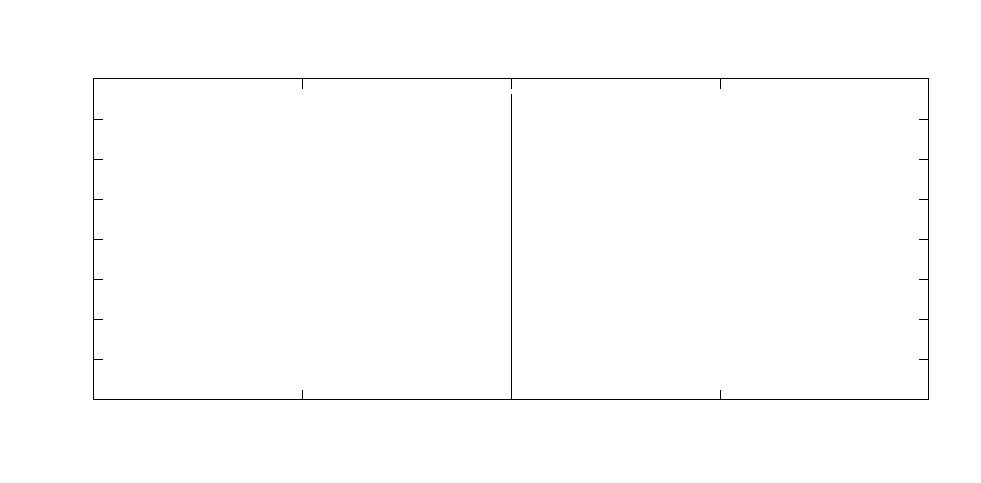
\includegraphics{local-calidad-testing}}%
    \gplfronttext
  \end{picture}%
\endgroup

\end{figure}

\begin{figure}[H]
	% GNUPLOT: LaTeX picture with Postscript
\begingroup
  \makeatletter
  \providecommand\color[2][]{%
    \GenericError{(gnuplot) \space\space\space\@spaces}{%
      Package color not loaded in conjunction with
      terminal option `colourtext'%
    }{See the gnuplot documentation for explanation.%
    }{Either use 'blacktext' in gnuplot or load the package
      color.sty in LaTeX.}%
    \renewcommand\color[2][]{}%
  }%
  \providecommand\includegraphics[2][]{%
    \GenericError{(gnuplot) \space\space\space\@spaces}{%
      Package graphicx or graphics not loaded%
    }{See the gnuplot documentation for explanation.%
    }{The gnuplot epslatex terminal needs graphicx.sty or graphics.sty.}%
    \renewcommand\includegraphics[2][]{}%
  }%
  \providecommand\rotatebox[2]{#2}%
  \@ifundefined{ifGPcolor}{%
    \newif\ifGPcolor
    \GPcolorfalse
  }{}%
  \@ifundefined{ifGPblacktext}{%
    \newif\ifGPblacktext
    \GPblacktexttrue
  }{}%
  % define a \g@addto@macro without @ in the name:
  \let\gplgaddtomacro\g@addto@macro
  % define empty templates for all commands taking text:
  \gdef\gplbacktext{}%
  \gdef\gplfronttext{}%
  \makeatother
  \ifGPblacktext
    % no textcolor at all
    \def\colorrgb#1{}%
    \def\colorgray#1{}%
  \else
    % gray or color?
    \ifGPcolor
      \def\colorrgb#1{\color[rgb]{#1}}%
      \def\colorgray#1{\color[gray]{#1}}%
      \expandafter\def\csname LTw\endcsname{\color{white}}%
      \expandafter\def\csname LTb\endcsname{\color{black}}%
      \expandafter\def\csname LTa\endcsname{\color{black}}%
      \expandafter\def\csname LT0\endcsname{\color[rgb]{1,0,0}}%
      \expandafter\def\csname LT1\endcsname{\color[rgb]{0,1,0}}%
      \expandafter\def\csname LT2\endcsname{\color[rgb]{0,0,1}}%
      \expandafter\def\csname LT3\endcsname{\color[rgb]{1,0,1}}%
      \expandafter\def\csname LT4\endcsname{\color[rgb]{0,1,1}}%
      \expandafter\def\csname LT5\endcsname{\color[rgb]{1,1,0}}%
      \expandafter\def\csname LT6\endcsname{\color[rgb]{0,0,0}}%
      \expandafter\def\csname LT7\endcsname{\color[rgb]{1,0.3,0}}%
      \expandafter\def\csname LT8\endcsname{\color[rgb]{0.5,0.5,0.5}}%
    \else
      % gray
      \def\colorrgb#1{\color{black}}%
      \def\colorgray#1{\color[gray]{#1}}%
      \expandafter\def\csname LTw\endcsname{\color{white}}%
      \expandafter\def\csname LTb\endcsname{\color{black}}%
      \expandafter\def\csname LTa\endcsname{\color{black}}%
      \expandafter\def\csname LT0\endcsname{\color{black}}%
      \expandafter\def\csname LT1\endcsname{\color{black}}%
      \expandafter\def\csname LT2\endcsname{\color{black}}%
      \expandafter\def\csname LT3\endcsname{\color{black}}%
      \expandafter\def\csname LT4\endcsname{\color{black}}%
      \expandafter\def\csname LT5\endcsname{\color{black}}%
      \expandafter\def\csname LT6\endcsname{\color{black}}%
      \expandafter\def\csname LT7\endcsname{\color{black}}%
      \expandafter\def\csname LT8\endcsname{\color{black}}%
    \fi
  \fi
  \setlength{\unitlength}{0.0500bp}%
  \begin{picture}(9118.00,4320.00)%
    \gplgaddtomacro\gplbacktext{%
      \colorrgb{0.00,0.00,0.00}%
      \put(620,640){\makebox(0,0)[r]{\strut{}0}}%
      \colorrgb{0.00,0.00,0.00}%
      \put(620,1153){\makebox(0,0)[r]{\strut{}5}}%
      \colorrgb{0.00,0.00,0.00}%
      \put(620,1666){\makebox(0,0)[r]{\strut{}10}}%
      \colorrgb{0.00,0.00,0.00}%
      \put(620,2180){\makebox(0,0)[r]{\strut{}15}}%
      \colorrgb{0.00,0.00,0.00}%
      \put(620,2693){\makebox(0,0)[r]{\strut{}20}}%
      \colorrgb{0.00,0.00,0.00}%
      \put(620,3206){\makebox(0,0)[r]{\strut{}25}}%
      \colorrgb{0.00,0.00,0.00}%
      \put(620,3719){\makebox(0,0)[r]{\strut{}30}}%
      \colorrgb{0.00,0.00,0.00}%
      \put(740,440){\makebox(0,0){\strut{}0}}%
      \colorrgb{0.00,0.00,0.00}%
      \put(2076,440){\makebox(0,0){\strut{}10}}%
      \colorrgb{0.00,0.00,0.00}%
      \put(3412,440){\makebox(0,0){\strut{}20}}%
      \colorrgb{0.00,0.00,0.00}%
      \put(4749,440){\makebox(0,0){\strut{}30}}%
      \colorrgb{0.00,0.00,0.00}%
      \put(6085,440){\makebox(0,0){\strut{}40}}%
      \colorrgb{0.00,0.00,0.00}%
      \put(7421,440){\makebox(0,0){\strut{}50}}%
      \colorrgb{0.00,0.00,0.00}%
      \put(8757,440){\makebox(0,0){\strut{}60}}%
      \colorrgb{0.00,0.00,0.00}%
      \put(160,2179){\rotatebox{90}{\makebox(0,0){\strut{}Frecuencia}}}%
      \colorrgb{0.00,0.00,0.00}%
      \put(4748,140){\makebox(0,0){\strut{}Tama\~no de la frontera: diferencia respecto de la soluci\'on exacta}}%
      \csname LTb\endcsname%
      \put(4748,4019){\makebox(0,0){\strut{}Heur\'istica Tab\'u: calidad de las soluciones}}%
    }%
    \gplgaddtomacro\gplfronttext{%
    }%
    \gplbacktext
    \put(0,0){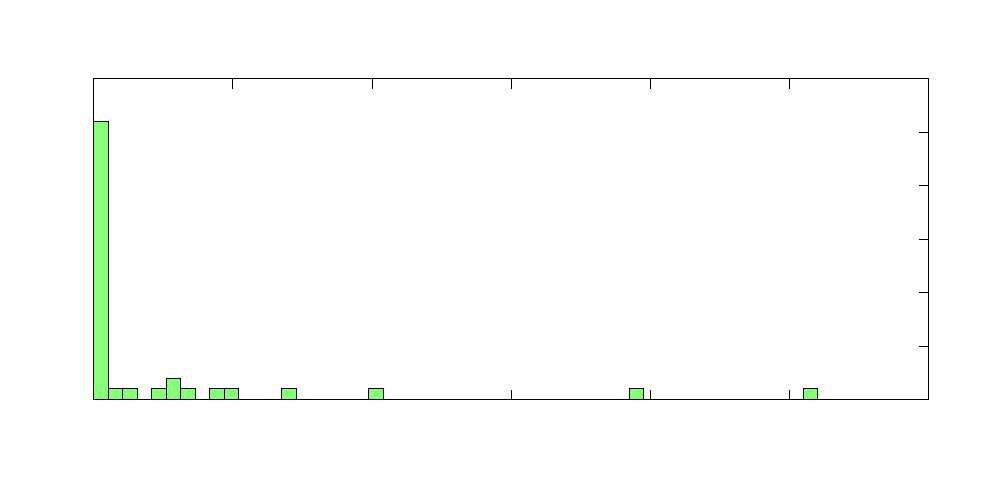
\includegraphics{tabu-calidad-testing}}%
    \gplfronttext
  \end{picture}%
\endgroup

\end{figure}


\subsubsection{Tiempo de ejecución}

\begin{figure}[H]
	% GNUPLOT: LaTeX picture with Postscript
\begingroup
  \makeatletter
  \providecommand\color[2][]{%
    \GenericError{(gnuplot) \space\space\space\@spaces}{%
      Package color not loaded in conjunction with
      terminal option `colourtext'%
    }{See the gnuplot documentation for explanation.%
    }{Either use 'blacktext' in gnuplot or load the package
      color.sty in LaTeX.}%
    \renewcommand\color[2][]{}%
  }%
  \providecommand\includegraphics[2][]{%
    \GenericError{(gnuplot) \space\space\space\@spaces}{%
      Package graphicx or graphics not loaded%
    }{See the gnuplot documentation for explanation.%
    }{The gnuplot epslatex terminal needs graphicx.sty or graphics.sty.}%
    \renewcommand\includegraphics[2][]{}%
  }%
  \providecommand\rotatebox[2]{#2}%
  \@ifundefined{ifGPcolor}{%
    \newif\ifGPcolor
    \GPcolorfalse
  }{}%
  \@ifundefined{ifGPblacktext}{%
    \newif\ifGPblacktext
    \GPblacktexttrue
  }{}%
  % define a \g@addto@macro without @ in the name:
  \let\gplgaddtomacro\g@addto@macro
  % define empty templates for all commands taking text:
  \gdef\gplbacktext{}%
  \gdef\gplfronttext{}%
  \makeatother
  \ifGPblacktext
    % no textcolor at all
    \def\colorrgb#1{}%
    \def\colorgray#1{}%
  \else
    % gray or color?
    \ifGPcolor
      \def\colorrgb#1{\color[rgb]{#1}}%
      \def\colorgray#1{\color[gray]{#1}}%
      \expandafter\def\csname LTw\endcsname{\color{white}}%
      \expandafter\def\csname LTb\endcsname{\color{black}}%
      \expandafter\def\csname LTa\endcsname{\color{black}}%
      \expandafter\def\csname LT0\endcsname{\color[rgb]{1,0,0}}%
      \expandafter\def\csname LT1\endcsname{\color[rgb]{0,1,0}}%
      \expandafter\def\csname LT2\endcsname{\color[rgb]{0,0,1}}%
      \expandafter\def\csname LT3\endcsname{\color[rgb]{1,0,1}}%
      \expandafter\def\csname LT4\endcsname{\color[rgb]{0,1,1}}%
      \expandafter\def\csname LT5\endcsname{\color[rgb]{1,1,0}}%
      \expandafter\def\csname LT6\endcsname{\color[rgb]{0,0,0}}%
      \expandafter\def\csname LT7\endcsname{\color[rgb]{1,0.3,0}}%
      \expandafter\def\csname LT8\endcsname{\color[rgb]{0.5,0.5,0.5}}%
    \else
      % gray
      \def\colorrgb#1{\color{black}}%
      \def\colorgray#1{\color[gray]{#1}}%
      \expandafter\def\csname LTw\endcsname{\color{white}}%
      \expandafter\def\csname LTb\endcsname{\color{black}}%
      \expandafter\def\csname LTa\endcsname{\color{black}}%
      \expandafter\def\csname LT0\endcsname{\color{black}}%
      \expandafter\def\csname LT1\endcsname{\color{black}}%
      \expandafter\def\csname LT2\endcsname{\color{black}}%
      \expandafter\def\csname LT3\endcsname{\color{black}}%
      \expandafter\def\csname LT4\endcsname{\color{black}}%
      \expandafter\def\csname LT5\endcsname{\color{black}}%
      \expandafter\def\csname LT6\endcsname{\color{black}}%
      \expandafter\def\csname LT7\endcsname{\color{black}}%
      \expandafter\def\csname LT8\endcsname{\color{black}}%
    \fi
  \fi
  \setlength{\unitlength}{0.0500bp}%
  \begin{picture}(9118.00,4320.00)%
    \gplgaddtomacro\gplbacktext{%
      \colorrgb{0.00,0.00,0.00}%
      \put(620,640){\makebox(0,0)[r]{\strut{}0}}%
      \colorrgb{0.00,0.00,0.00}%
      \put(620,1256){\makebox(0,0)[r]{\strut{}5}}%
      \colorrgb{0.00,0.00,0.00}%
      \put(620,1872){\makebox(0,0)[r]{\strut{}10}}%
      \colorrgb{0.00,0.00,0.00}%
      \put(620,2487){\makebox(0,0)[r]{\strut{}15}}%
      \colorrgb{0.00,0.00,0.00}%
      \put(620,3103){\makebox(0,0)[r]{\strut{}20}}%
      \colorrgb{0.00,0.00,0.00}%
      \put(620,3719){\makebox(0,0)[r]{\strut{}25}}%
      \colorrgb{0.00,0.00,0.00}%
      \put(740,440){\makebox(0,0){\strut{}0.011}}%
      \colorrgb{0.00,0.00,0.00}%
      \put(1742,440){\makebox(0,0){\strut{}0.0115}}%
      \colorrgb{0.00,0.00,0.00}%
      \put(2744,440){\makebox(0,0){\strut{}0.012}}%
      \colorrgb{0.00,0.00,0.00}%
      \put(3746,440){\makebox(0,0){\strut{}0.0125}}%
      \colorrgb{0.00,0.00,0.00}%
      \put(4749,440){\makebox(0,0){\strut{}0.013}}%
      \colorrgb{0.00,0.00,0.00}%
      \put(5751,440){\makebox(0,0){\strut{}0.0135}}%
      \colorrgb{0.00,0.00,0.00}%
      \put(6753,440){\makebox(0,0){\strut{}0.014}}%
      \colorrgb{0.00,0.00,0.00}%
      \put(7755,440){\makebox(0,0){\strut{}0.0145}}%
      \colorrgb{0.00,0.00,0.00}%
      \put(8757,440){\makebox(0,0){\strut{}0.015}}%
      \colorrgb{0.00,0.00,0.00}%
      \put(160,2179){\rotatebox{90}{\makebox(0,0){\strut{}Frecuencia}}}%
      \colorrgb{0.00,0.00,0.00}%
      \put(4748,140){\makebox(0,0){\strut{}Tiempo de ejecuci\'on (milisegundos)}}%
      \csname LTb\endcsname%
      \put(4748,4019){\makebox(0,0){\strut{}Heur\'istica Golosa: tiempo de ejecuci\'on}}%
    }%
    \gplgaddtomacro\gplfronttext{%
    }%
    \gplbacktext
    \put(0,0){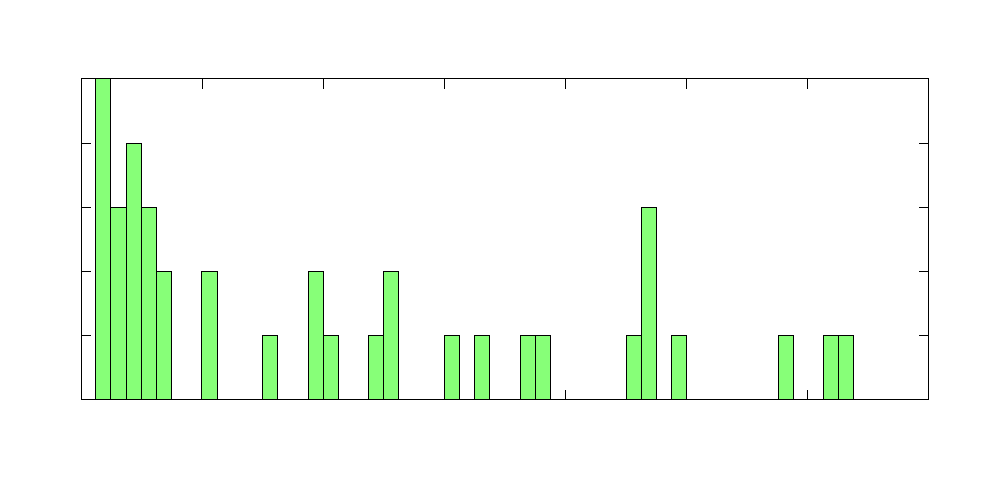
\includegraphics{golosa-tiempo-testing}}%
    \gplfronttext
  \end{picture}%
\endgroup

\end{figure}

\begin{figure}[H]
	% GNUPLOT: LaTeX picture with Postscript
\begingroup
  \makeatletter
  \providecommand\color[2][]{%
    \GenericError{(gnuplot) \space\space\space\@spaces}{%
      Package color not loaded in conjunction with
      terminal option `colourtext'%
    }{See the gnuplot documentation for explanation.%
    }{Either use 'blacktext' in gnuplot or load the package
      color.sty in LaTeX.}%
    \renewcommand\color[2][]{}%
  }%
  \providecommand\includegraphics[2][]{%
    \GenericError{(gnuplot) \space\space\space\@spaces}{%
      Package graphicx or graphics not loaded%
    }{See the gnuplot documentation for explanation.%
    }{The gnuplot epslatex terminal needs graphicx.sty or graphics.sty.}%
    \renewcommand\includegraphics[2][]{}%
  }%
  \providecommand\rotatebox[2]{#2}%
  \@ifundefined{ifGPcolor}{%
    \newif\ifGPcolor
    \GPcolorfalse
  }{}%
  \@ifundefined{ifGPblacktext}{%
    \newif\ifGPblacktext
    \GPblacktexttrue
  }{}%
  % define a \g@addto@macro without @ in the name:
  \let\gplgaddtomacro\g@addto@macro
  % define empty templates for all commands taking text:
  \gdef\gplbacktext{}%
  \gdef\gplfronttext{}%
  \makeatother
  \ifGPblacktext
    % no textcolor at all
    \def\colorrgb#1{}%
    \def\colorgray#1{}%
  \else
    % gray or color?
    \ifGPcolor
      \def\colorrgb#1{\color[rgb]{#1}}%
      \def\colorgray#1{\color[gray]{#1}}%
      \expandafter\def\csname LTw\endcsname{\color{white}}%
      \expandafter\def\csname LTb\endcsname{\color{black}}%
      \expandafter\def\csname LTa\endcsname{\color{black}}%
      \expandafter\def\csname LT0\endcsname{\color[rgb]{1,0,0}}%
      \expandafter\def\csname LT1\endcsname{\color[rgb]{0,1,0}}%
      \expandafter\def\csname LT2\endcsname{\color[rgb]{0,0,1}}%
      \expandafter\def\csname LT3\endcsname{\color[rgb]{1,0,1}}%
      \expandafter\def\csname LT4\endcsname{\color[rgb]{0,1,1}}%
      \expandafter\def\csname LT5\endcsname{\color[rgb]{1,1,0}}%
      \expandafter\def\csname LT6\endcsname{\color[rgb]{0,0,0}}%
      \expandafter\def\csname LT7\endcsname{\color[rgb]{1,0.3,0}}%
      \expandafter\def\csname LT8\endcsname{\color[rgb]{0.5,0.5,0.5}}%
    \else
      % gray
      \def\colorrgb#1{\color{black}}%
      \def\colorgray#1{\color[gray]{#1}}%
      \expandafter\def\csname LTw\endcsname{\color{white}}%
      \expandafter\def\csname LTb\endcsname{\color{black}}%
      \expandafter\def\csname LTa\endcsname{\color{black}}%
      \expandafter\def\csname LT0\endcsname{\color{black}}%
      \expandafter\def\csname LT1\endcsname{\color{black}}%
      \expandafter\def\csname LT2\endcsname{\color{black}}%
      \expandafter\def\csname LT3\endcsname{\color{black}}%
      \expandafter\def\csname LT4\endcsname{\color{black}}%
      \expandafter\def\csname LT5\endcsname{\color{black}}%
      \expandafter\def\csname LT6\endcsname{\color{black}}%
      \expandafter\def\csname LT7\endcsname{\color{black}}%
      \expandafter\def\csname LT8\endcsname{\color{black}}%
    \fi
  \fi
  \setlength{\unitlength}{0.0500bp}%
  \begin{picture}(9118.00,4320.00)%
    \gplgaddtomacro\gplbacktext{%
      \colorrgb{0.00,0.00,0.00}%
      \put(500,640){\makebox(0,0)[r]{\strut{}0}}%
      \colorrgb{0.00,0.00,0.00}%
      \put(500,1153){\makebox(0,0)[r]{\strut{}1}}%
      \colorrgb{0.00,0.00,0.00}%
      \put(500,1666){\makebox(0,0)[r]{\strut{}2}}%
      \colorrgb{0.00,0.00,0.00}%
      \put(500,2180){\makebox(0,0)[r]{\strut{}3}}%
      \colorrgb{0.00,0.00,0.00}%
      \put(500,2693){\makebox(0,0)[r]{\strut{}4}}%
      \colorrgb{0.00,0.00,0.00}%
      \put(500,3206){\makebox(0,0)[r]{\strut{}5}}%
      \colorrgb{0.00,0.00,0.00}%
      \put(500,3719){\makebox(0,0)[r]{\strut{}6}}%
      \colorrgb{0.00,0.00,0.00}%
      \put(620,440){\makebox(0,0){\strut{}0}}%
      \colorrgb{0.00,0.00,0.00}%
      \put(2247,440){\makebox(0,0){\strut{}0.2}}%
      \colorrgb{0.00,0.00,0.00}%
      \put(3875,440){\makebox(0,0){\strut{}0.4}}%
      \colorrgb{0.00,0.00,0.00}%
      \put(5502,440){\makebox(0,0){\strut{}0.6}}%
      \colorrgb{0.00,0.00,0.00}%
      \put(7130,440){\makebox(0,0){\strut{}0.8}}%
      \colorrgb{0.00,0.00,0.00}%
      \put(8757,440){\makebox(0,0){\strut{}1}}%
      \colorrgb{0.00,0.00,0.00}%
      \put(160,2179){\rotatebox{90}{\makebox(0,0){\strut{}Frecuencia}}}%
      \colorrgb{0.00,0.00,0.00}%
      \put(4688,140){\makebox(0,0){\strut{}Tiempo de ejecuci\'on (milisegundos)}}%
      \csname LTb\endcsname%
      \put(4688,4019){\makebox(0,0){\strut{}Heur\'istica Local: tiempo de ejecuci\'on}}%
    }%
    \gplgaddtomacro\gplfronttext{%
    }%
    \gplbacktext
    \put(0,0){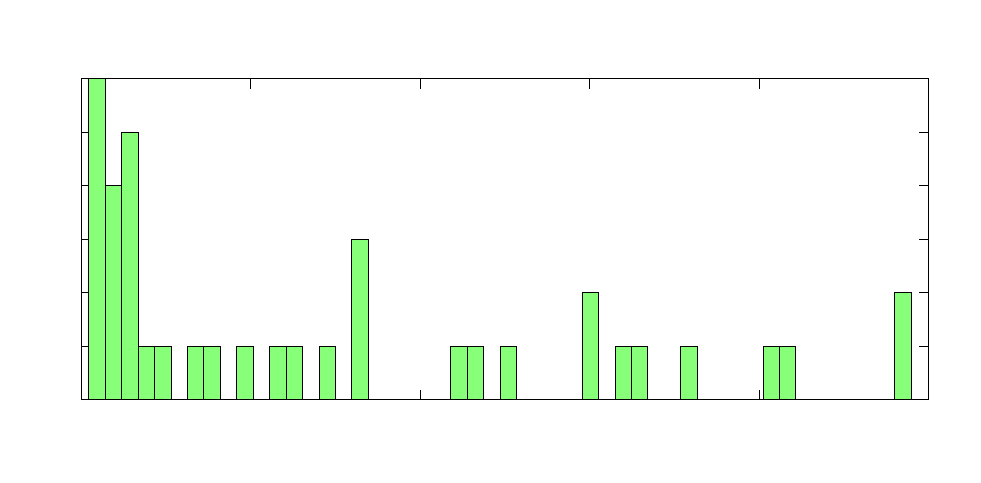
\includegraphics{local-tiempo-testing}}%
    \gplfronttext
  \end{picture}%
\endgroup

\end{figure}

\begin{figure}[H]
	% GNUPLOT: LaTeX picture with Postscript
\begingroup
  \makeatletter
  \providecommand\color[2][]{%
    \GenericError{(gnuplot) \space\space\space\@spaces}{%
      Package color not loaded in conjunction with
      terminal option `colourtext'%
    }{See the gnuplot documentation for explanation.%
    }{Either use 'blacktext' in gnuplot or load the package
      color.sty in LaTeX.}%
    \renewcommand\color[2][]{}%
  }%
  \providecommand\includegraphics[2][]{%
    \GenericError{(gnuplot) \space\space\space\@spaces}{%
      Package graphicx or graphics not loaded%
    }{See the gnuplot documentation for explanation.%
    }{The gnuplot epslatex terminal needs graphicx.sty or graphics.sty.}%
    \renewcommand\includegraphics[2][]{}%
  }%
  \providecommand\rotatebox[2]{#2}%
  \@ifundefined{ifGPcolor}{%
    \newif\ifGPcolor
    \GPcolorfalse
  }{}%
  \@ifundefined{ifGPblacktext}{%
    \newif\ifGPblacktext
    \GPblacktexttrue
  }{}%
  % define a \g@addto@macro without @ in the name:
  \let\gplgaddtomacro\g@addto@macro
  % define empty templates for all commands taking text:
  \gdef\gplbacktext{}%
  \gdef\gplfronttext{}%
  \makeatother
  \ifGPblacktext
    % no textcolor at all
    \def\colorrgb#1{}%
    \def\colorgray#1{}%
  \else
    % gray or color?
    \ifGPcolor
      \def\colorrgb#1{\color[rgb]{#1}}%
      \def\colorgray#1{\color[gray]{#1}}%
      \expandafter\def\csname LTw\endcsname{\color{white}}%
      \expandafter\def\csname LTb\endcsname{\color{black}}%
      \expandafter\def\csname LTa\endcsname{\color{black}}%
      \expandafter\def\csname LT0\endcsname{\color[rgb]{1,0,0}}%
      \expandafter\def\csname LT1\endcsname{\color[rgb]{0,1,0}}%
      \expandafter\def\csname LT2\endcsname{\color[rgb]{0,0,1}}%
      \expandafter\def\csname LT3\endcsname{\color[rgb]{1,0,1}}%
      \expandafter\def\csname LT4\endcsname{\color[rgb]{0,1,1}}%
      \expandafter\def\csname LT5\endcsname{\color[rgb]{1,1,0}}%
      \expandafter\def\csname LT6\endcsname{\color[rgb]{0,0,0}}%
      \expandafter\def\csname LT7\endcsname{\color[rgb]{1,0.3,0}}%
      \expandafter\def\csname LT8\endcsname{\color[rgb]{0.5,0.5,0.5}}%
    \else
      % gray
      \def\colorrgb#1{\color{black}}%
      \def\colorgray#1{\color[gray]{#1}}%
      \expandafter\def\csname LTw\endcsname{\color{white}}%
      \expandafter\def\csname LTb\endcsname{\color{black}}%
      \expandafter\def\csname LTa\endcsname{\color{black}}%
      \expandafter\def\csname LT0\endcsname{\color{black}}%
      \expandafter\def\csname LT1\endcsname{\color{black}}%
      \expandafter\def\csname LT2\endcsname{\color{black}}%
      \expandafter\def\csname LT3\endcsname{\color{black}}%
      \expandafter\def\csname LT4\endcsname{\color{black}}%
      \expandafter\def\csname LT5\endcsname{\color{black}}%
      \expandafter\def\csname LT6\endcsname{\color{black}}%
      \expandafter\def\csname LT7\endcsname{\color{black}}%
      \expandafter\def\csname LT8\endcsname{\color{black}}%
    \fi
  \fi
  \setlength{\unitlength}{0.0500bp}%
  \begin{picture}(9118.00,4320.00)%
    \gplgaddtomacro\gplbacktext{%
      \colorrgb{0.00,0.00,0.00}%
      \put(620,640){\makebox(0,0)[r]{\strut{}0}}%
      \colorrgb{0.00,0.00,0.00}%
      \put(620,1080){\makebox(0,0)[r]{\strut{}2}}%
      \colorrgb{0.00,0.00,0.00}%
      \put(620,1520){\makebox(0,0)[r]{\strut{}4}}%
      \colorrgb{0.00,0.00,0.00}%
      \put(620,1960){\makebox(0,0)[r]{\strut{}6}}%
      \colorrgb{0.00,0.00,0.00}%
      \put(620,2399){\makebox(0,0)[r]{\strut{}8}}%
      \colorrgb{0.00,0.00,0.00}%
      \put(620,2839){\makebox(0,0)[r]{\strut{}10}}%
      \colorrgb{0.00,0.00,0.00}%
      \put(620,3279){\makebox(0,0)[r]{\strut{}12}}%
      \colorrgb{0.00,0.00,0.00}%
      \put(620,3719){\makebox(0,0)[r]{\strut{}14}}%
      \colorrgb{0.00,0.00,0.00}%
      \put(740,440){\makebox(0,0){\strut{}0}}%
      \colorrgb{0.00,0.00,0.00}%
      \put(2343,440){\makebox(0,0){\strut{}2}}%
      \colorrgb{0.00,0.00,0.00}%
      \put(3947,440){\makebox(0,0){\strut{}4}}%
      \colorrgb{0.00,0.00,0.00}%
      \put(5550,440){\makebox(0,0){\strut{}6}}%
      \colorrgb{0.00,0.00,0.00}%
      \put(7154,440){\makebox(0,0){\strut{}8}}%
      \colorrgb{0.00,0.00,0.00}%
      \put(8757,440){\makebox(0,0){\strut{}10}}%
      \colorrgb{0.00,0.00,0.00}%
      \put(160,2179){\rotatebox{90}{\makebox(0,0){\strut{}Frecuencia}}}%
      \colorrgb{0.00,0.00,0.00}%
      \put(4748,140){\makebox(0,0){\strut{}Tiempo de ejecuci\'on (milisegundos)}}%
      \csname LTb\endcsname%
      \put(4748,4019){\makebox(0,0){\strut{}Heur\'istica Tab\'u: tiempo de ejecuci\'on}}%
    }%
    \gplgaddtomacro\gplfronttext{%
    }%
    \gplbacktext
    \put(0,0){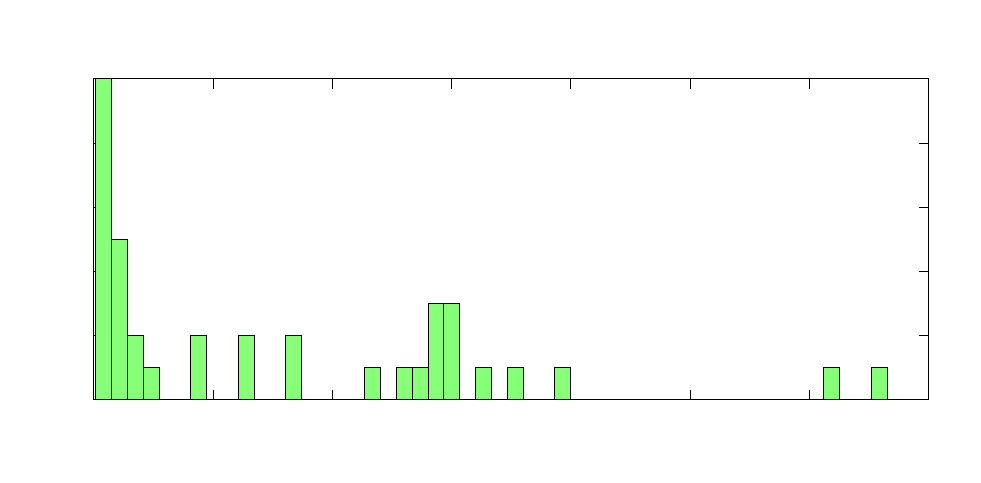
\includegraphics{tabu-tiempo-testing}}%
    \gplfronttext
  \end{picture}%
\endgroup

\end{figure}


\subsection{Estadísticas}

Las siguientes estadísticas sintetizan los resultados anteriores. Se tabulan la media ($\mu$) y desvío estándar ($\sigma$) para las siguientes métricas:

\begin{description}
	\item[Calidad:] diferencia entre el tamaño de la frontera de la solución hallada y la solución exacta.
	\item[Tiempo:] tiempo de ejecución de la heurística medido en milisegundos.
\end{description}

\newcommand{\golosaentrenamientocalidadmu}{0.3000}
\newcommand{\golosaentrenamientocalidadsigma}{1.4933}
\newcommand{\golosaentrenamientotiempomu}{0.0247}
\newcommand{\golosaentrenamientotiemposigma}{0.0262}
\newcommand{\golosatestingcalidadmu}{8.7105}
\newcommand{\golosatestingcalidadsigma}{15.5822}
\newcommand{\golosatestingtiempomu}{0.0949}
\newcommand{\golosatestingtiemposigma}{0.0948}

\newcommand{\localentrenamientocalidadmu}{0.3000}
\newcommand{\localentrenamientocalidadsigma}{1.4933}
\newcommand{\localentrenamientotiempomu}{0.0591}
\newcommand{\localentrenamientotiemposigma}{0.0718}
\newcommand{\localtestingcalidadmu}{8.7105}
\newcommand{\localtestingcalidadsigma}{15.5822}
\newcommand{\localtestingtiempomu}{0.3402}
\newcommand{\localtestingtiemposigma}{0.3475}

\newcommand{\tabuentrenamientocalidadmu}{0.0585}
\newcommand{\tabuentrenamientocalidadsigma}{0.4494}
\newcommand{\tabuentrenamientotiempomu}{0.2681}
\newcommand{\tabuentrenamientotiemposigma}{0.3929}
\newcommand{\tabutestingcalidadmu}{4.7368}
\newcommand{\tabutestingcalidadsigma}{10.8670}
\newcommand{\tabutestingtiempomu}{1.5997}
\newcommand{\tabutestingtiemposigma}{1.8702}



\begin{figure}[H]
	\begin{tabularx}{\textwidth}{ |>{\small}X| *9{ >{\small\centering}X|} }
		\hline
		\multirow{3}{*}{Heurística} &
		\multicolumn{4}{ l| }{Grafos de entrenamiento} &
		\multicolumn{4}{ l| }{Grafos de testing}
		\tabularnewline
		
		\cline{2-9}
		&
		\multicolumn{2}{ l| }{Calidad} &
		\multicolumn{2}{ l| }{Tiempo} &
		\multicolumn{2}{ l| }{Calidad} &
		\multicolumn{2}{ l| }{Tiempo}
		\tabularnewline

		\cline{2-9}
		& $\mu$ & $\sigma$ & $\mu$ & $\sigma$ & $\mu$ & $\sigma$ & $\mu$ & $\sigma$
		\tabularnewline

		\hline
		Golosa &
		\golosaentrenamientocalidadmu &
		\golosaentrenamientocalidadsigma &
		\golosaentrenamientotiempomu &
		\golosaentrenamientotiemposigma &
		\golosatestingcalidadmu &
		\golosatestingcalidadsigma &
		\golosatestingtiempomu &
		\golosatestingtiemposigma
		\tabularnewline

		\hline
		Local &
		\localentrenamientocalidadmu &
		\localentrenamientocalidadsigma &
		\localentrenamientotiempomu &
		\localentrenamientotiemposigma &
		\localtestingcalidadmu &
		\localtestingcalidadsigma &
		\localtestingtiempomu &
		\localtestingtiemposigma
		\tabularnewline

		\hline
		Tabú &
		\tabuentrenamientocalidadmu &
		\tabuentrenamientocalidadsigma &
		\tabuentrenamientotiempomu &
		\tabuentrenamientotiemposigma &
		\tabutestingcalidadmu &
		\tabutestingcalidadsigma &
		\tabutestingtiempomu &
		\tabutestingtiemposigma
		\tabularnewline

		\hline
	\end{tabularx}
\end{figure}

\end{document}